\documentclass[11pt,a4paper]{article}

\usepackage{graphicx}
\graphicspath{{res/}}

\usepackage{wrapfig}
\usepackage{titling}
\usepackage{fancyhdr}
\usepackage{minted}

\usepackage{geometry}
\geometry{
 a4paper,
 left=30mm,
 right=30mm,
 bottom=30mm,
 top=30mm,
 }

\title{Implement complex procedures to make a specified product using a Computer Numerical Controlled (CNC) machine 91622}
\author{Drew Bryan}
\date{2026}

\fancypagestyle{plain}{
    \fancyhf{}
    \fancyfoot[R]{\thepage}
    \fancyhead[L]{91622}
    \fancyhead[R]{\theauthor}
    \setlength{\headheight}{13.6pt}
}


\begin{document}
\pagestyle{plain}

\maketitle

\noindent
Equipment in the media studies department frequently goes lost. As a member of the Publicity Committee, I set out to make a small device to would sit in a closet that would manage who had what equipment.

\section{Design}

I used Fusion 360 to design my CAD model. I made real world measurements using callipers of the electronic components that would need to fit inside of it (LCD, RFID reader/writer), as well as my hand so it could be held comfortably. I used these measurements in my sketches which created my 3D geometry.

\begin{center}
    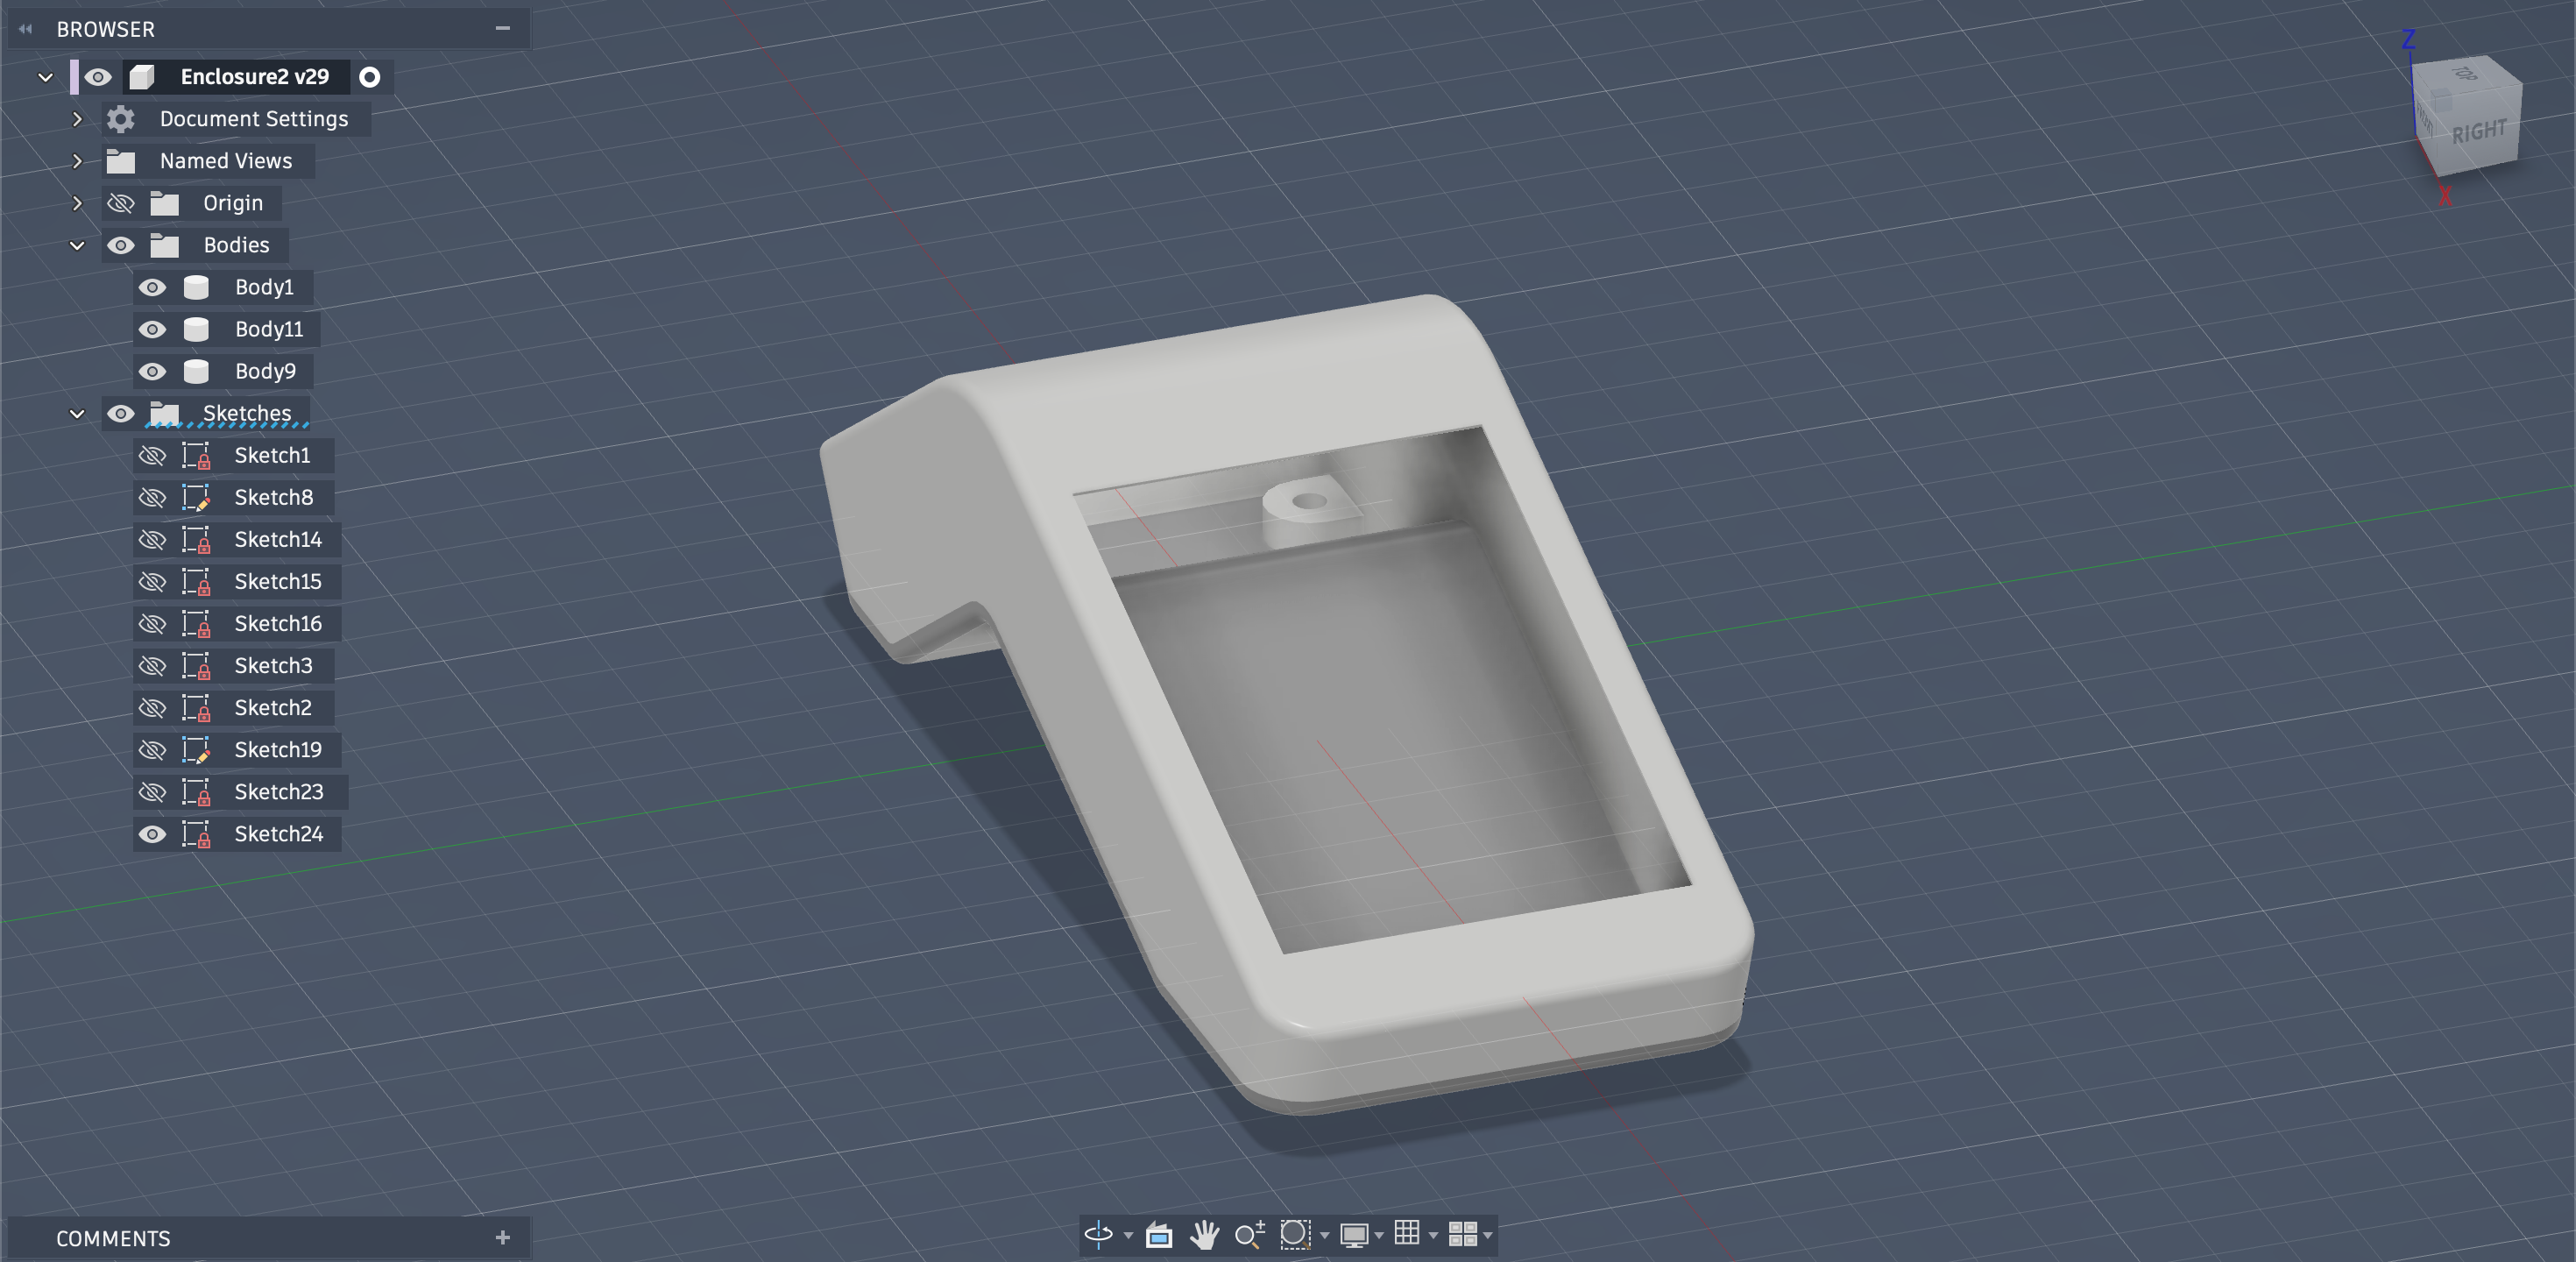
\includegraphics[width=0.49\textwidth]{model}
    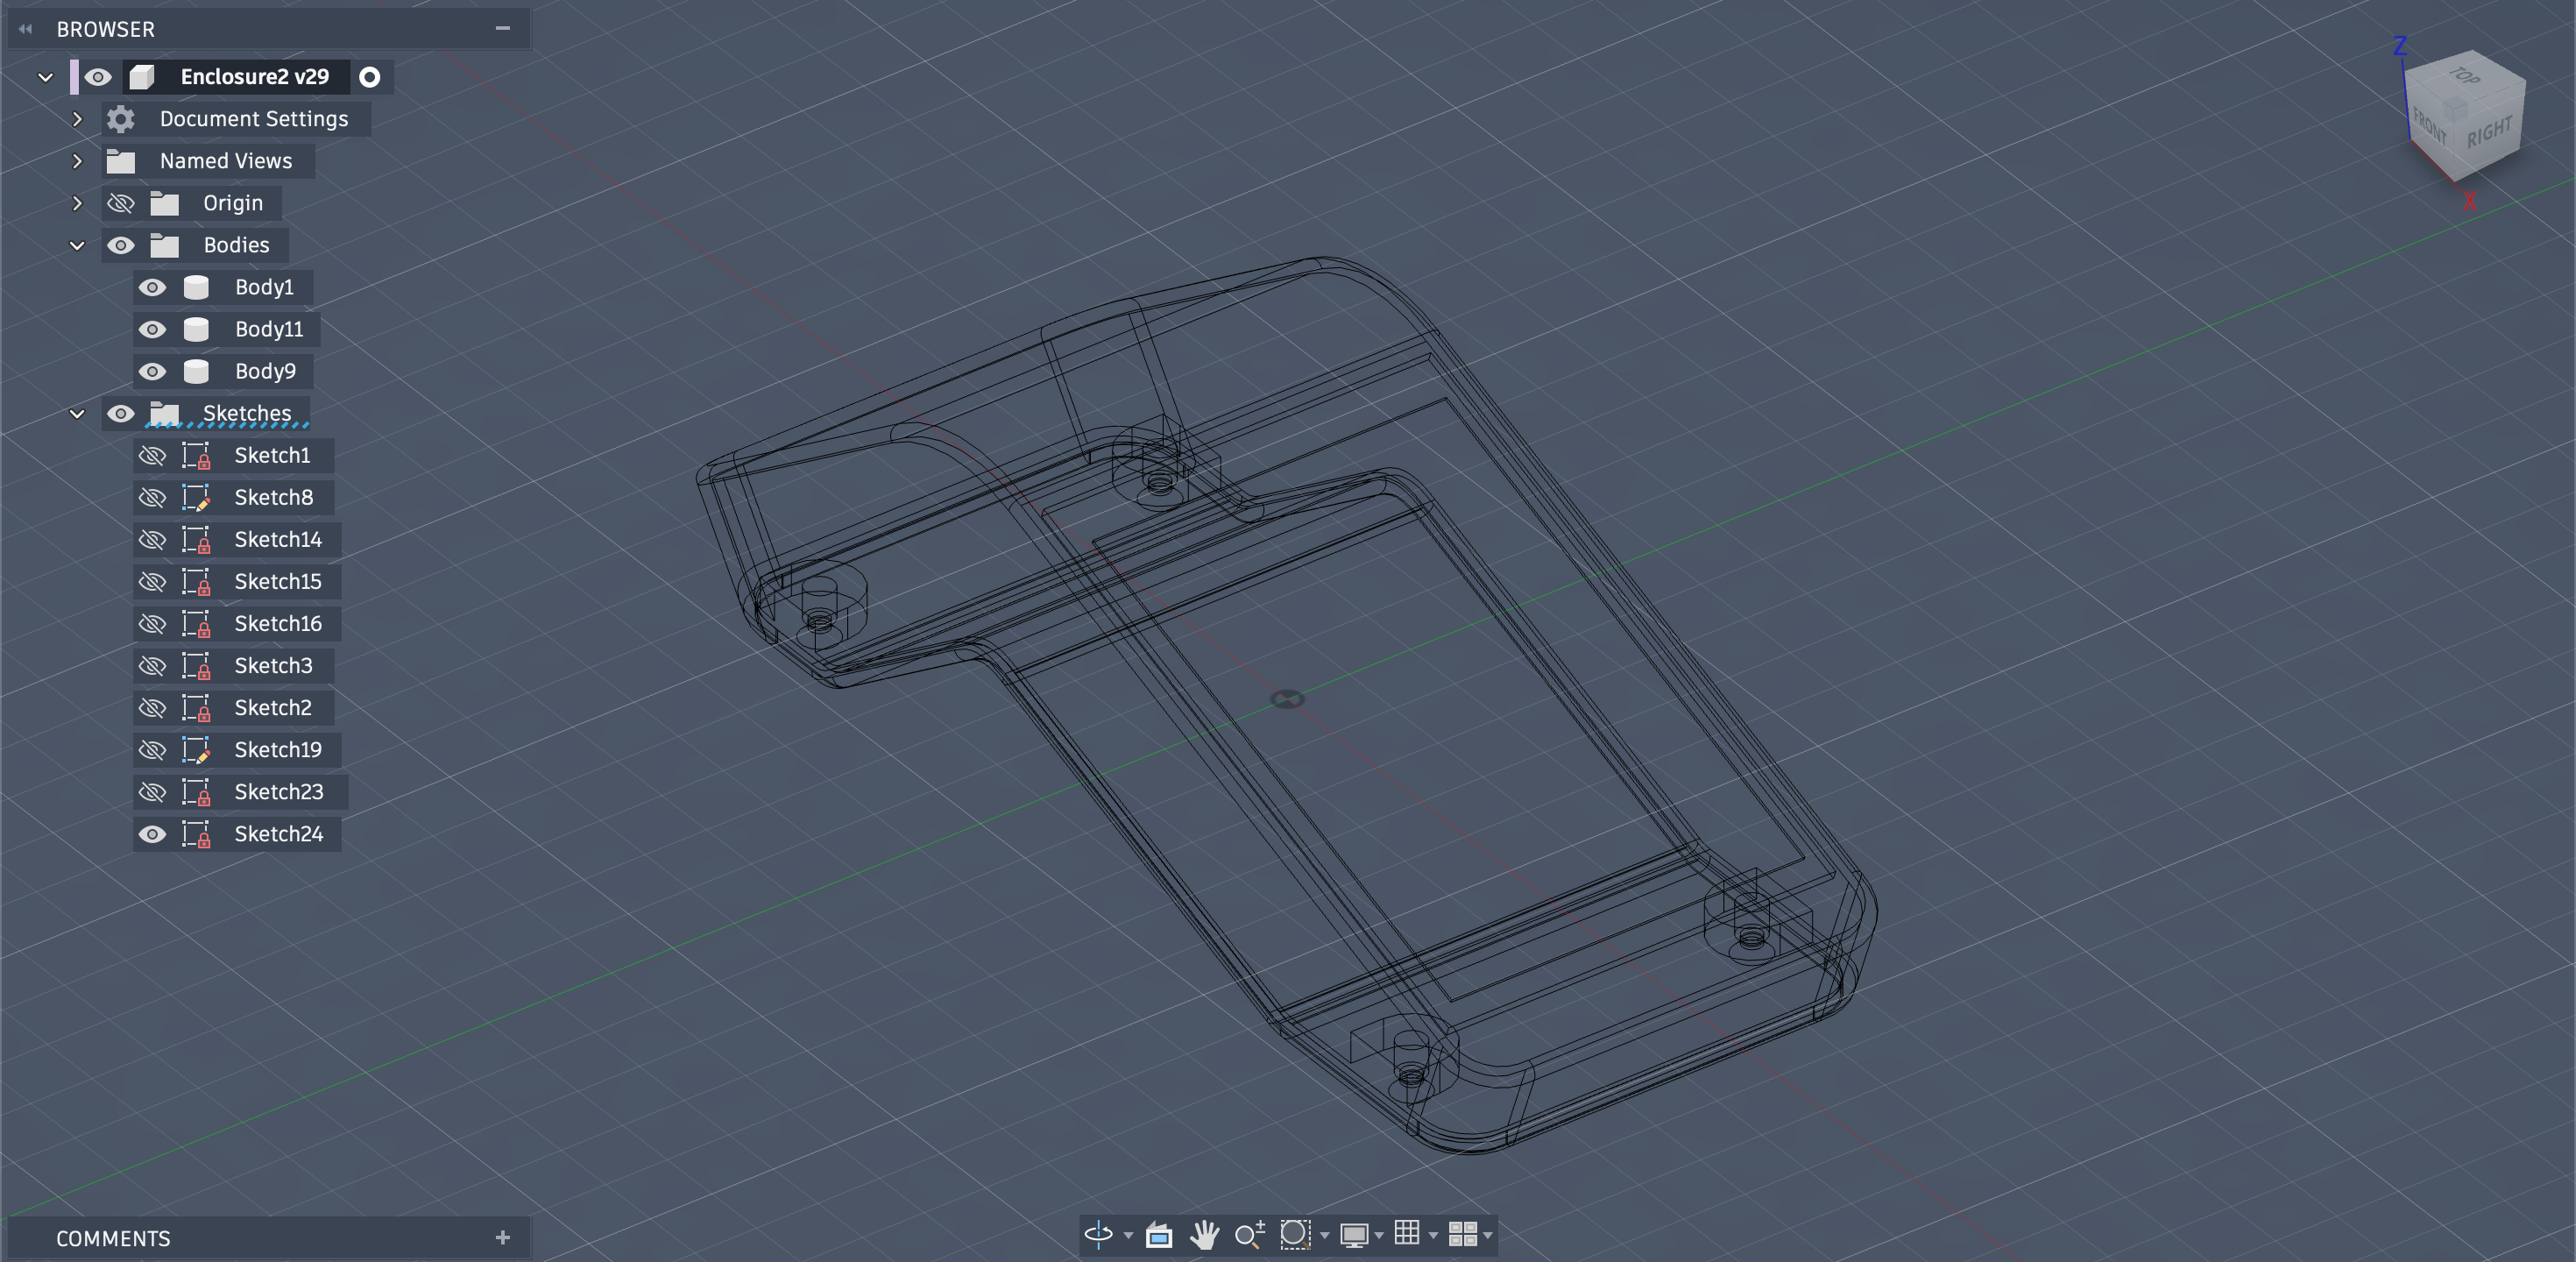
\includegraphics[width=0.49\textwidth]{model_wireframe}
\end{center}

\begin{wrapfigure}{r}{0.4\textwidth}
    \centering
    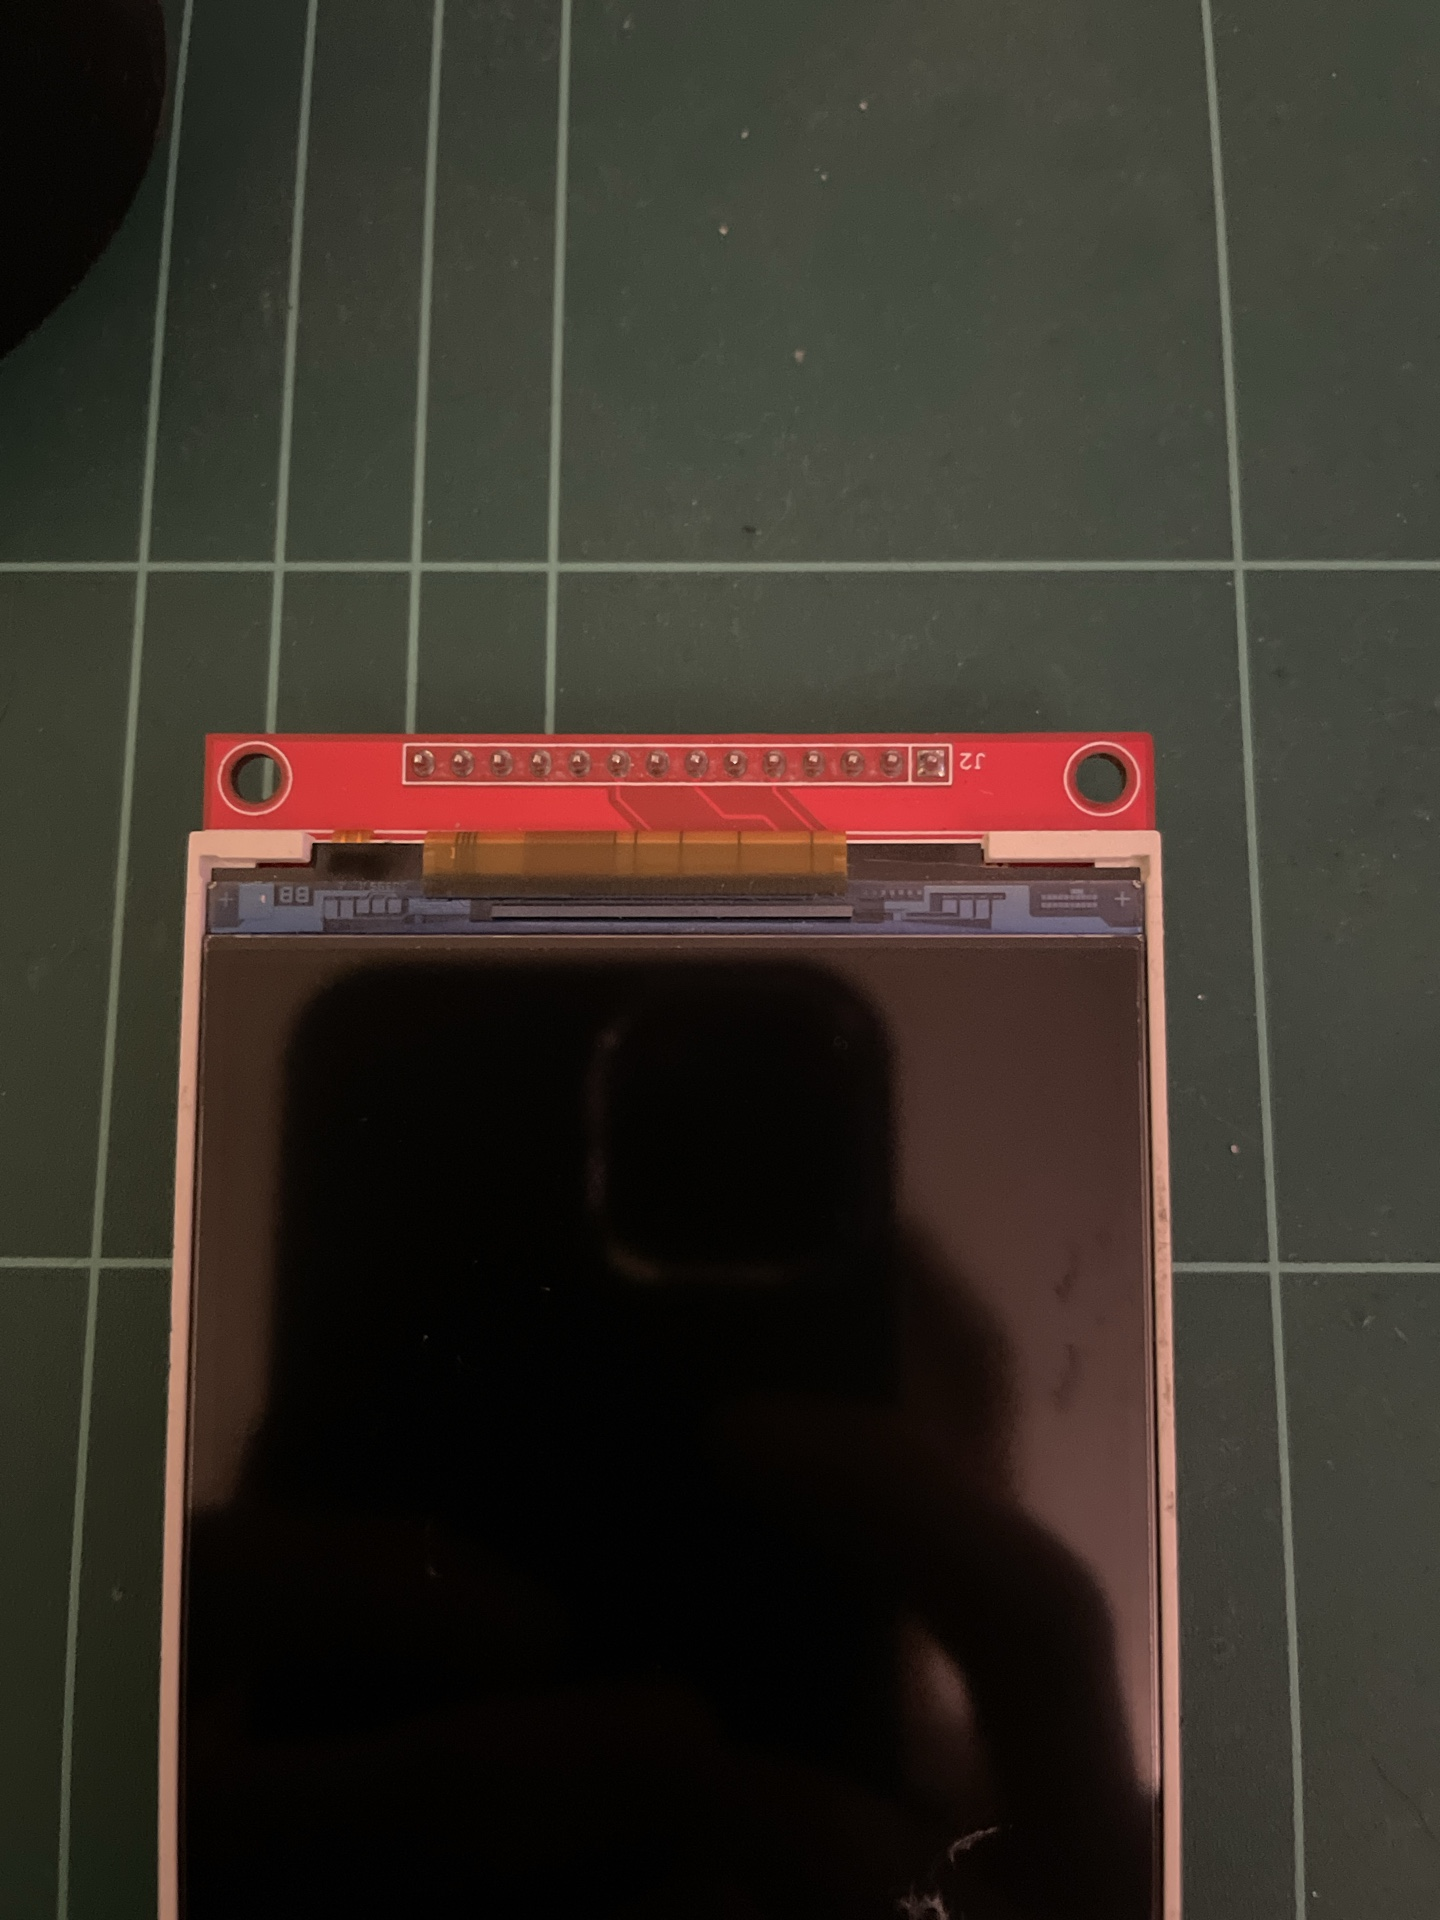
\includegraphics[width=0.35\textwidth, trim=0px 300px 0px 0px, clip]{screen_notch}
\end{wrapfigure}

\noindent
I paid close attention to all the details to make sure that my components would fit properly and that it would look premium from the outside. One of the details that I needed to consider was that the viewable area of the LCD screen that I am using has a notch at the top. I created a small rectangle cutout for this notch to fit into so the screen could be close to flush with the shell.

No fabricator is perfect, and so I had to consider tolerances when copying my measurements. I had to add tolerances to many parts, but one of them was for the outer white rectangle of the screen, to fit in the rectangle cutout. I measured $94.5\times61$mm but added 0.5mm to each dimension to make sure that it would fit. I also created minimal overhangs in the design for maximum print orientation flexibility, so I can decrease the time and material I have to use by using less supports. There are also other limitations of a 3D printer, including build volume and resolution, which were not very relevant to my design since it does not contain any micro-features and is small well small enough to fit in the build volume of my printer.

\begin{figure}[ht]
    \centering
    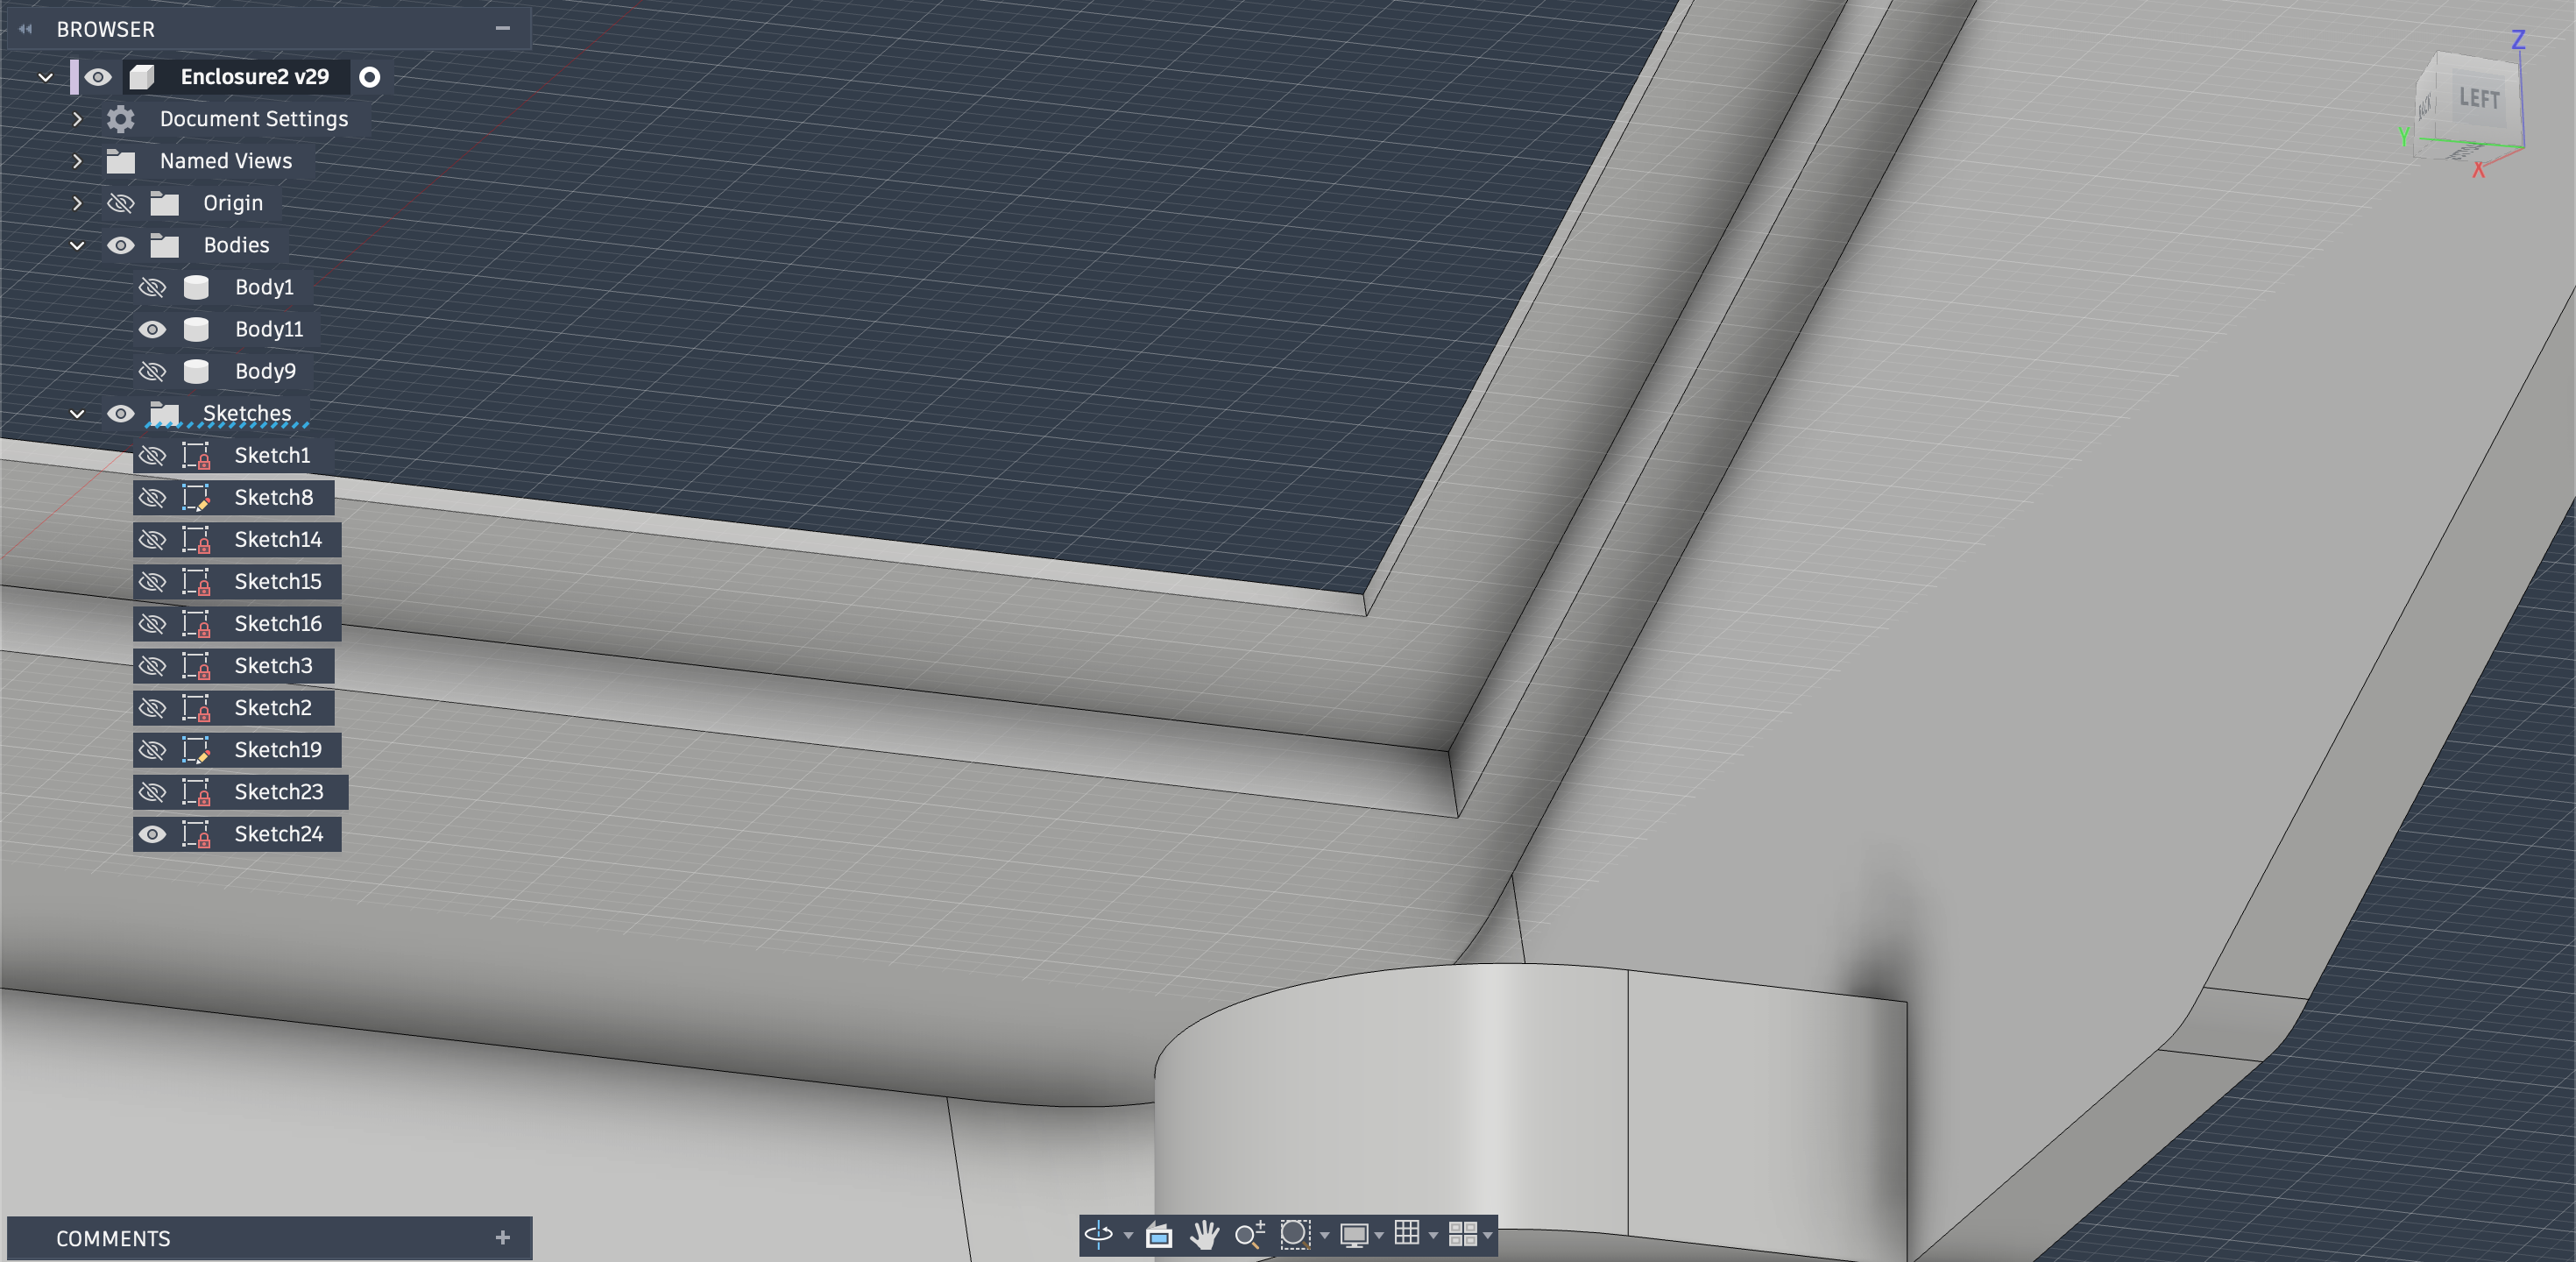
\includegraphics[width=1\textwidth]{cutout}
    \caption{Rectangle cutout}
\end{figure}

\section{Setup}

To operate a 3D printer, there are some preparation steps that need to be done, one of which is generating the instructions that the printer interprets and performs (gcode). This is referred to as `slicing' because the model is split up into layers. Some other steps, including bed leveling and loading filament are also required.

\subsection{Slicing}

The model of my printer is a Bambu Lab P1S, and so to slice my models into gcode I use Bambu Studio because it can wirelessly start my prints.

After creating a project you can import 3D models or generate primitives. A view of the plate can be used to place and orient objects. This is the first piece of configuration that you encounter in the slicer since the orientation of an object has large implications on the strength and flexibility of the outcome.

\begin{figure}[ht]
    \centering
    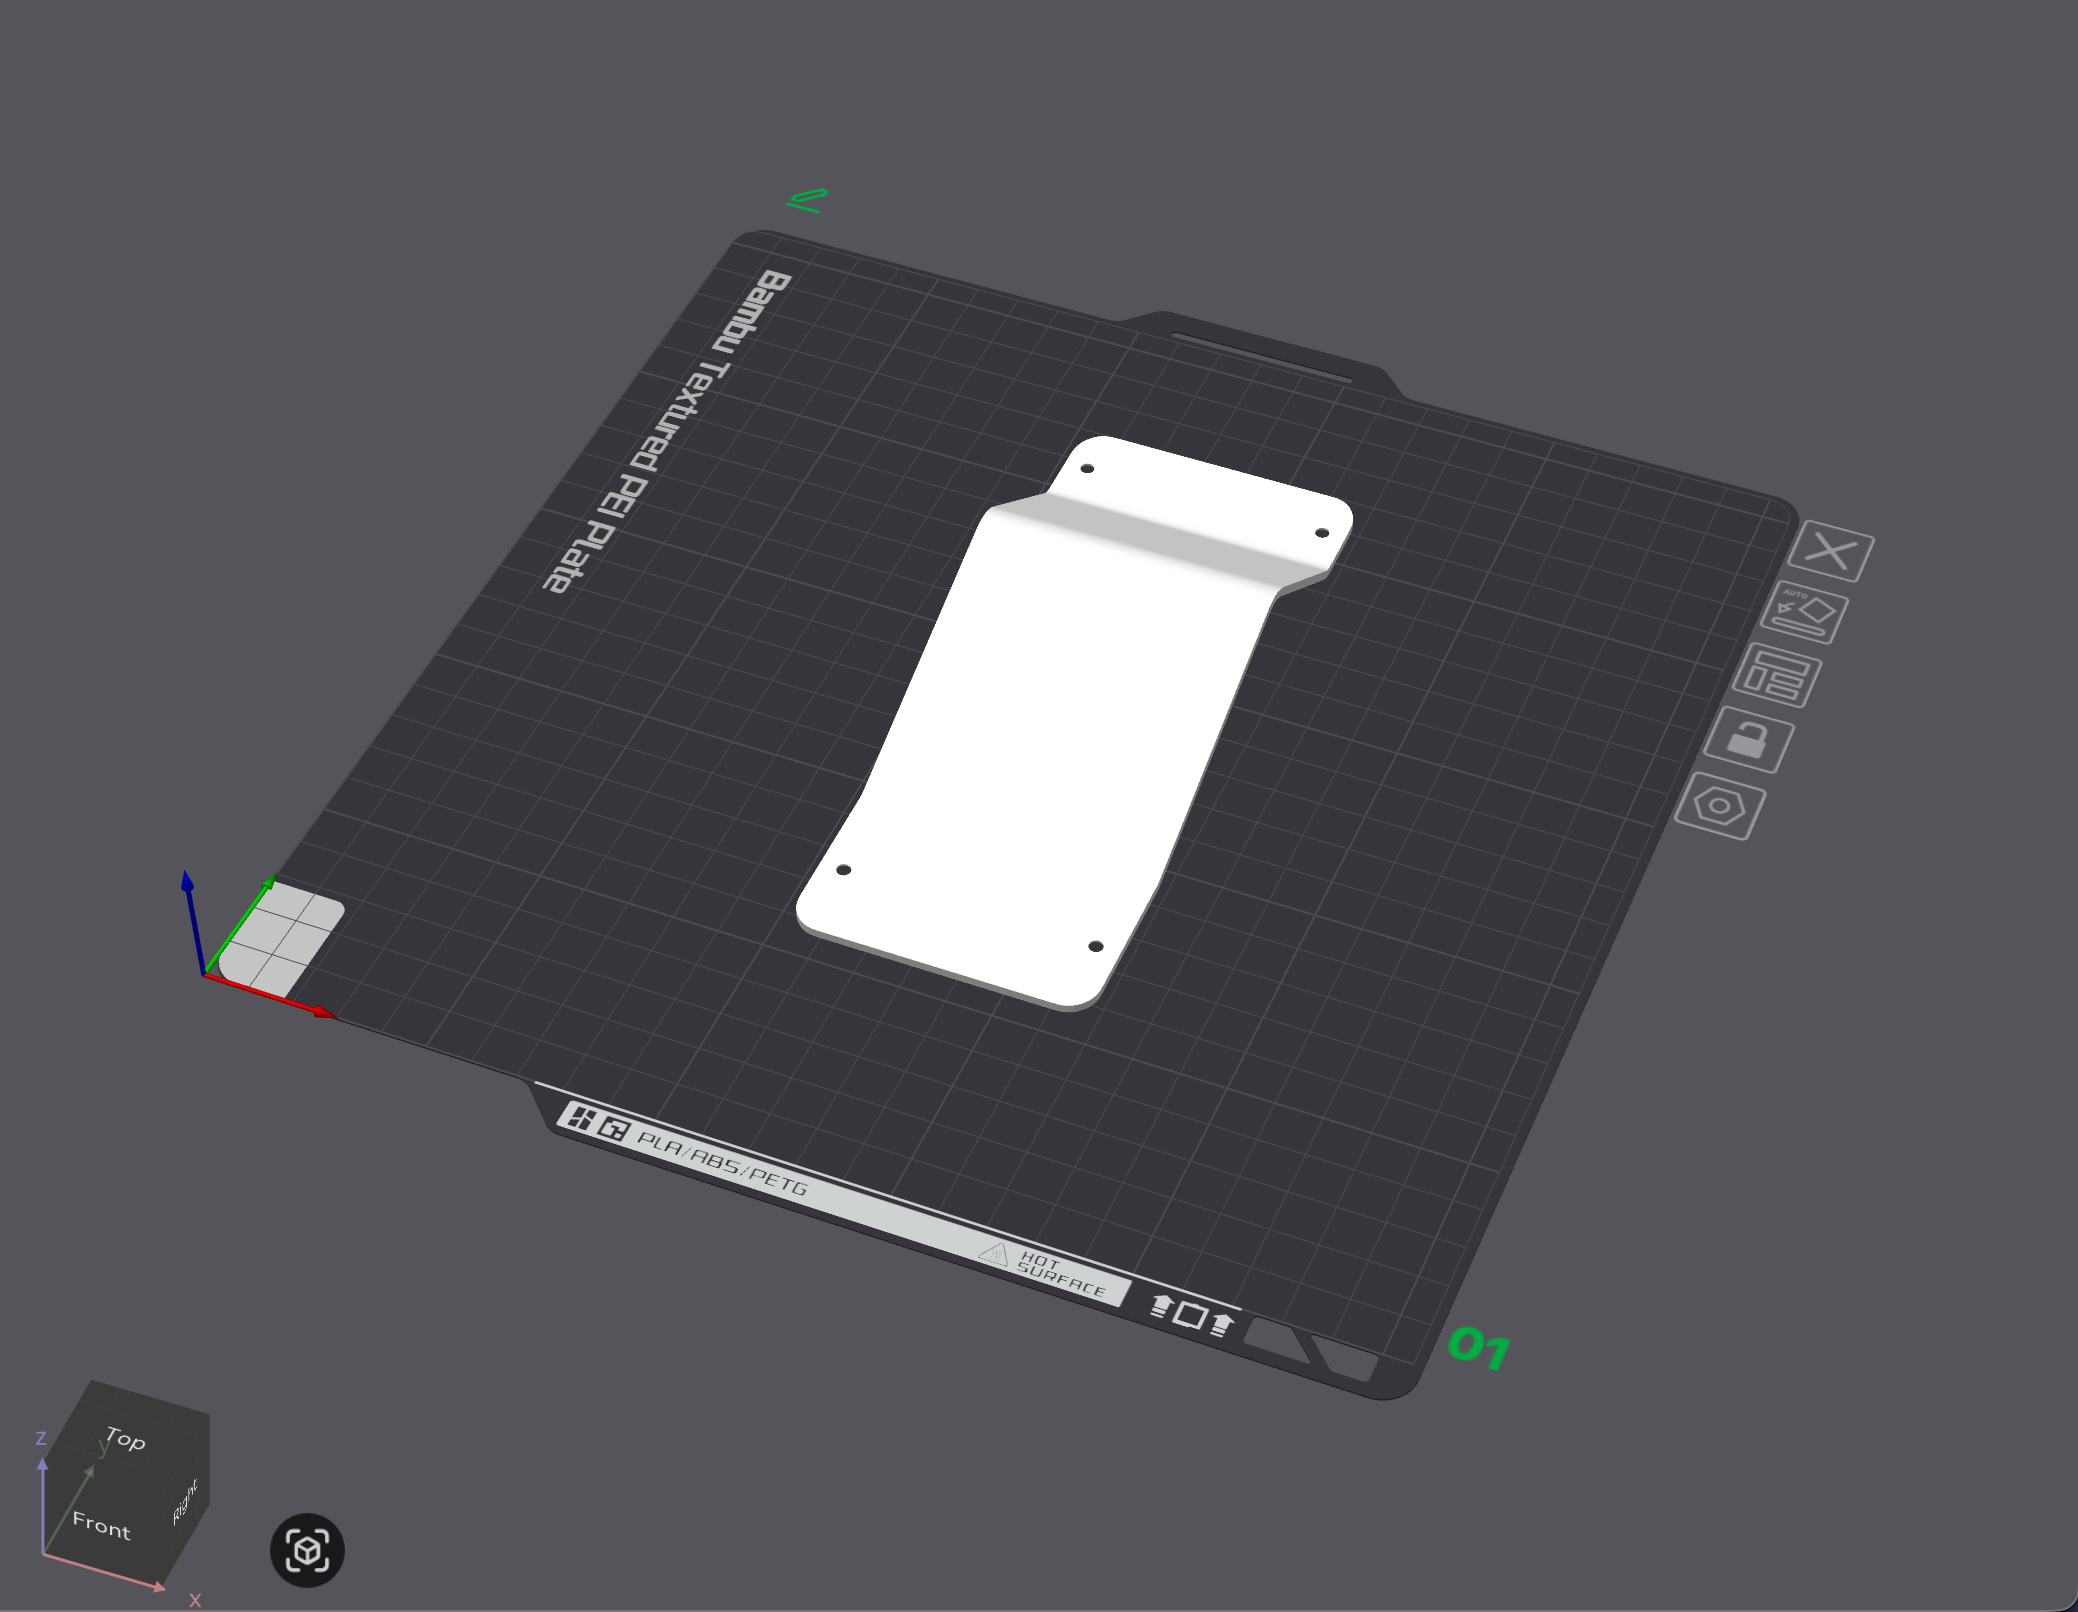
\includegraphics[width=0.49\textwidth]{flat_orientation}
    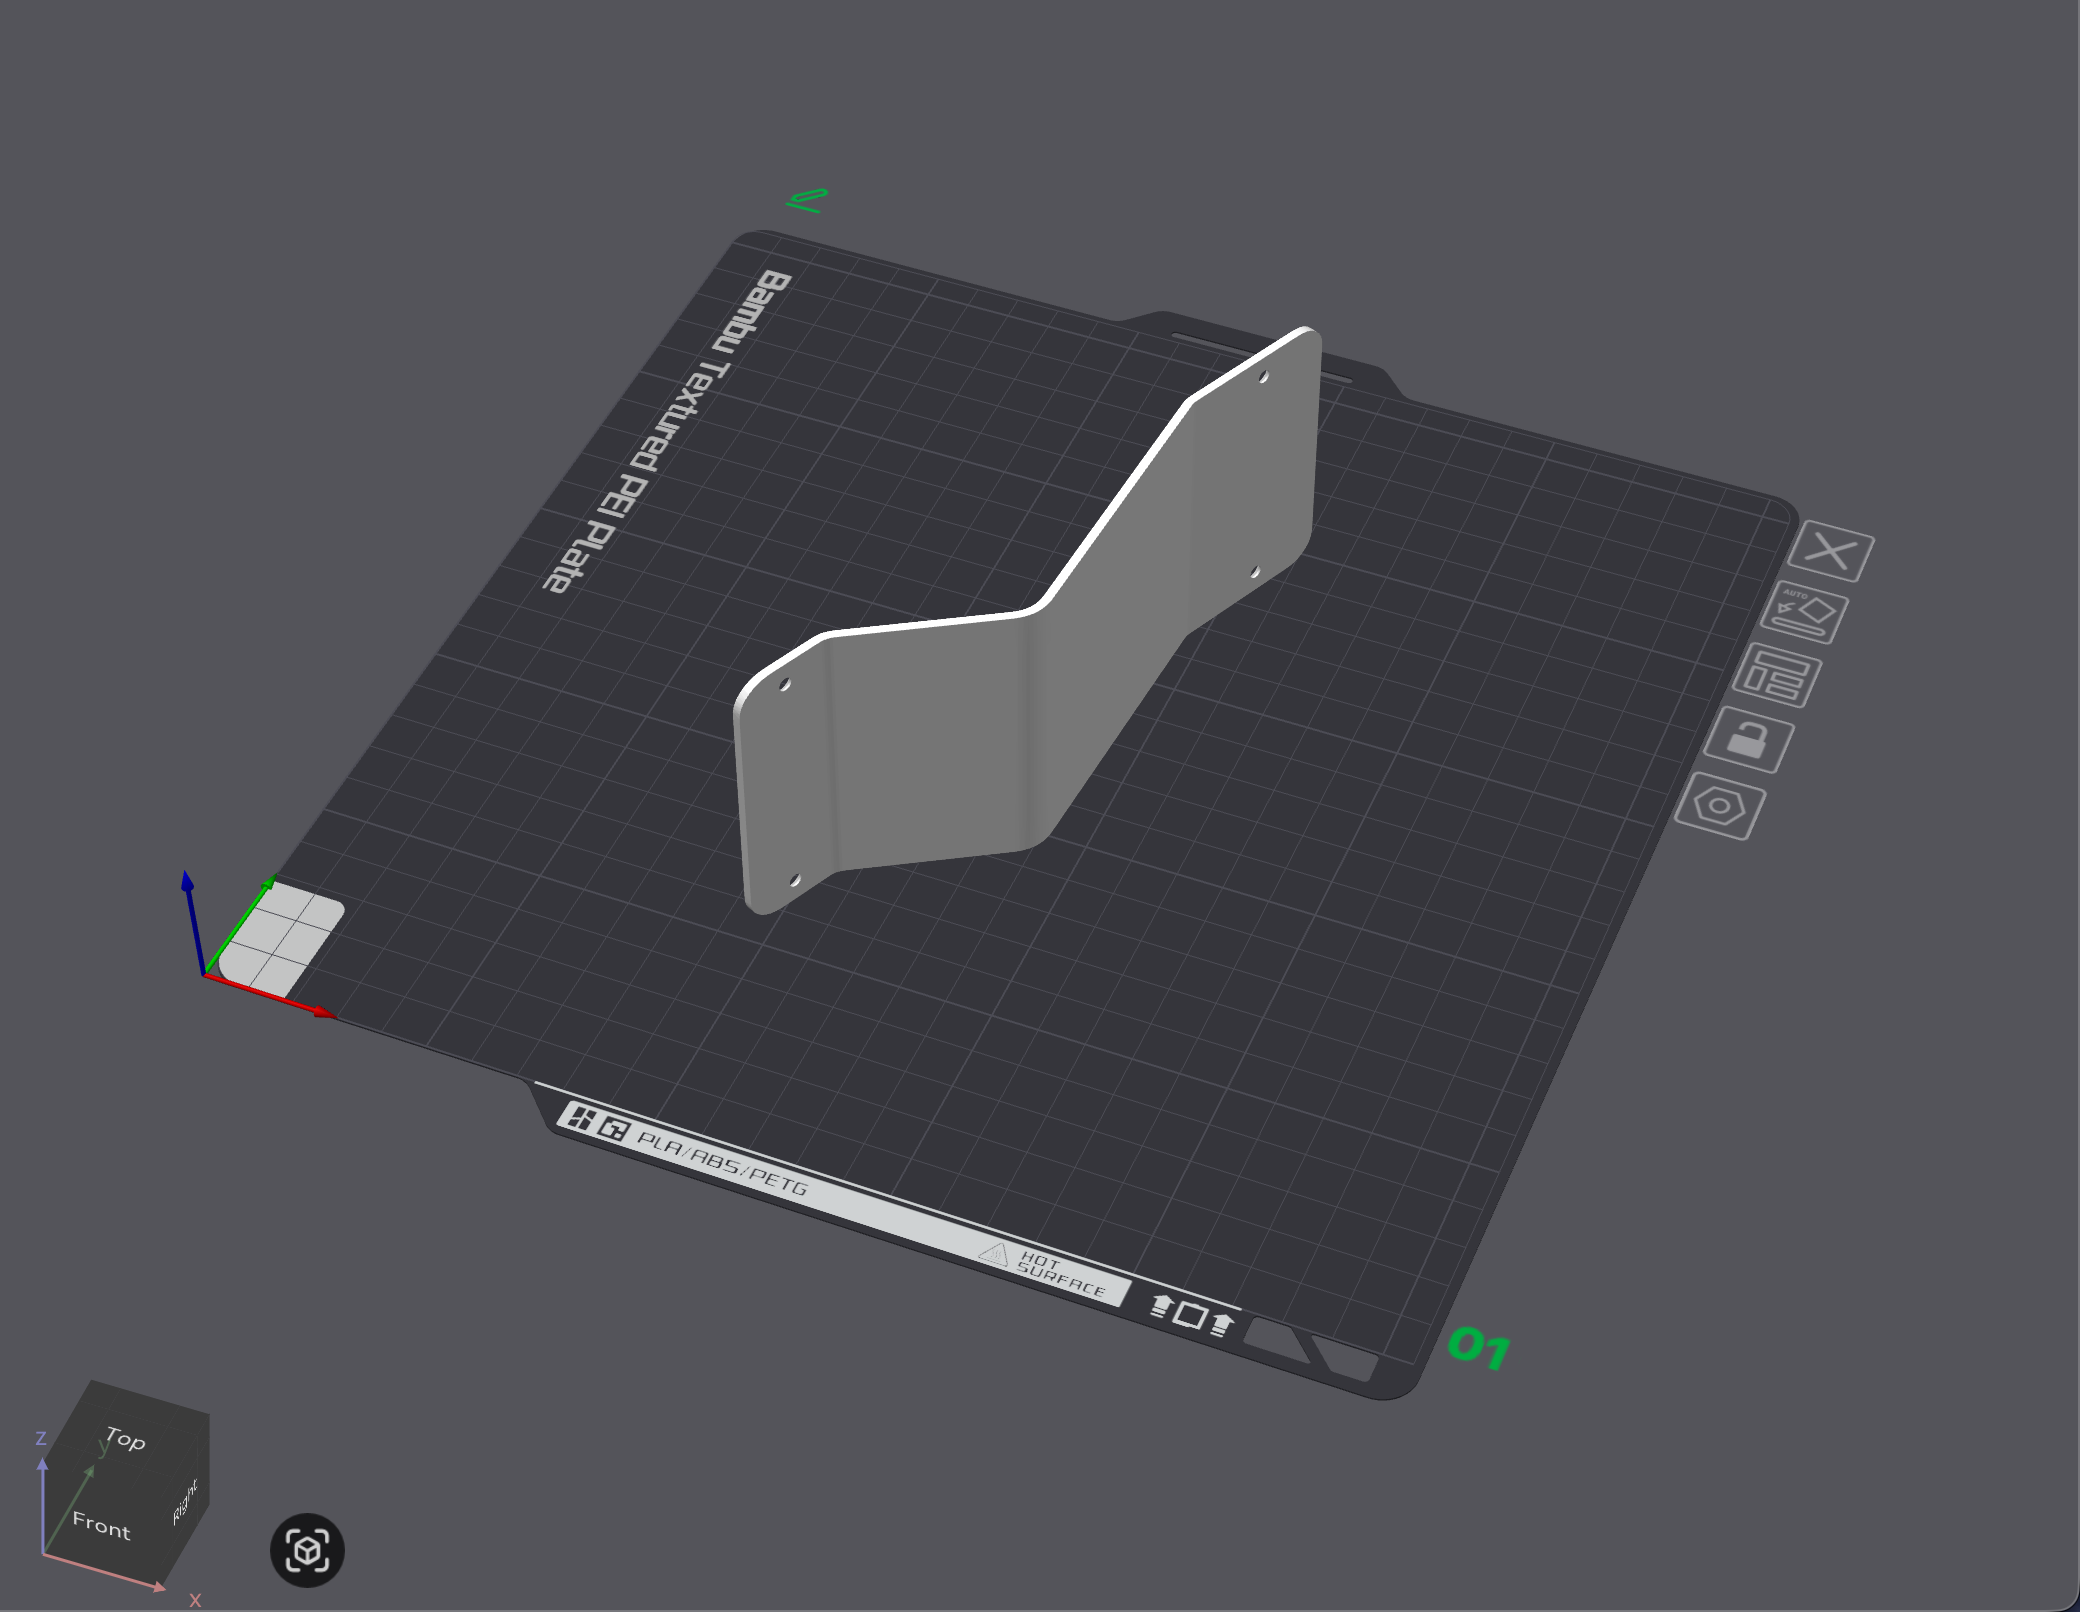
\includegraphics[width=0.49\textwidth]{tall_orientation}
    \caption{Alternative orientations}\label{fig:orientations}
\end{figure}

\noindent
A printed object is much more prone to snapping along the layer lines and bends perpendicular to the layers. This is why, in my case, the right orientation in figure~\ref{fig:orientations} is preferred.

The position of the object also matters to optimise speed and travel distance, or if you are printing in object mode instead of layer mode (which prints all the layers of an object before switching to the next object) because the objects need to be spaced enough for the toolhead print on the bed.

\bigbreak\noindent
Some commonly changed settings relating to the strength are the infill and wall loops. The wall loops is the number of times that the wall will be traced, making it thicker. The infill however, has both a pattern and percentage that can be changed, among other, less significant settings. The pattern will change what is drawn inside of the walls, and the percentage will change the frequency of the pattern relative to the amount of space available (100\% is solid).

\begin{figure}[ht]
    \centering
    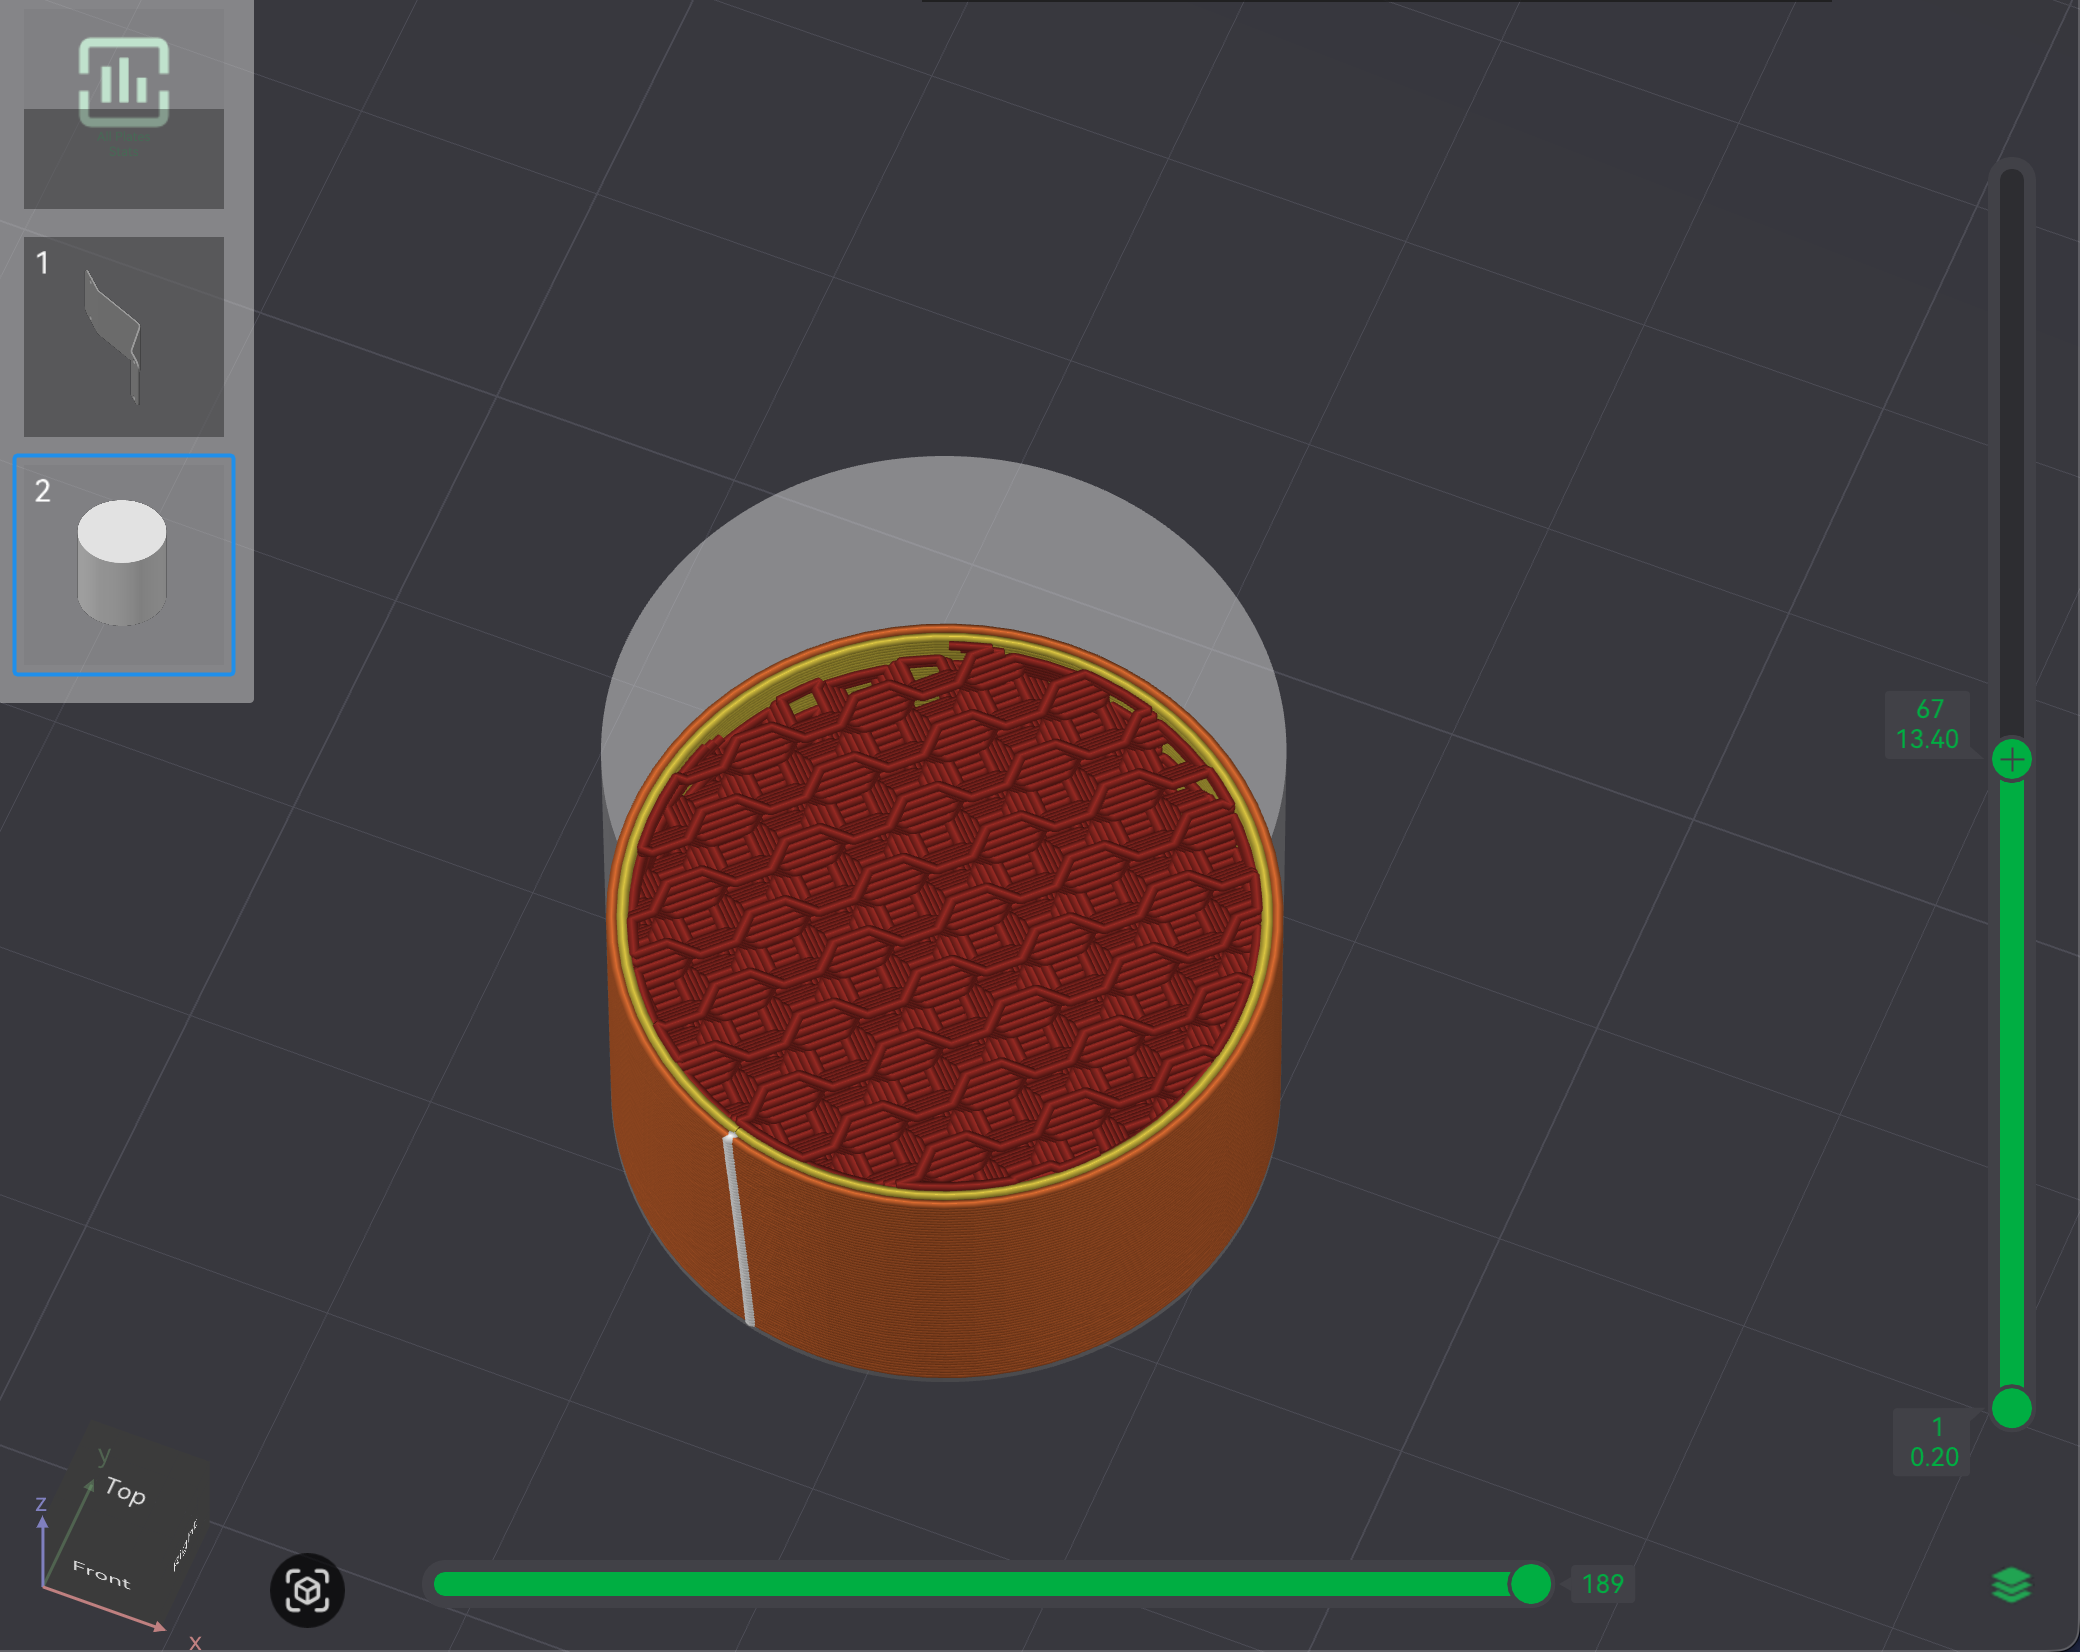
\includegraphics[width=0.49\textwidth]{3dhoneycomb}
    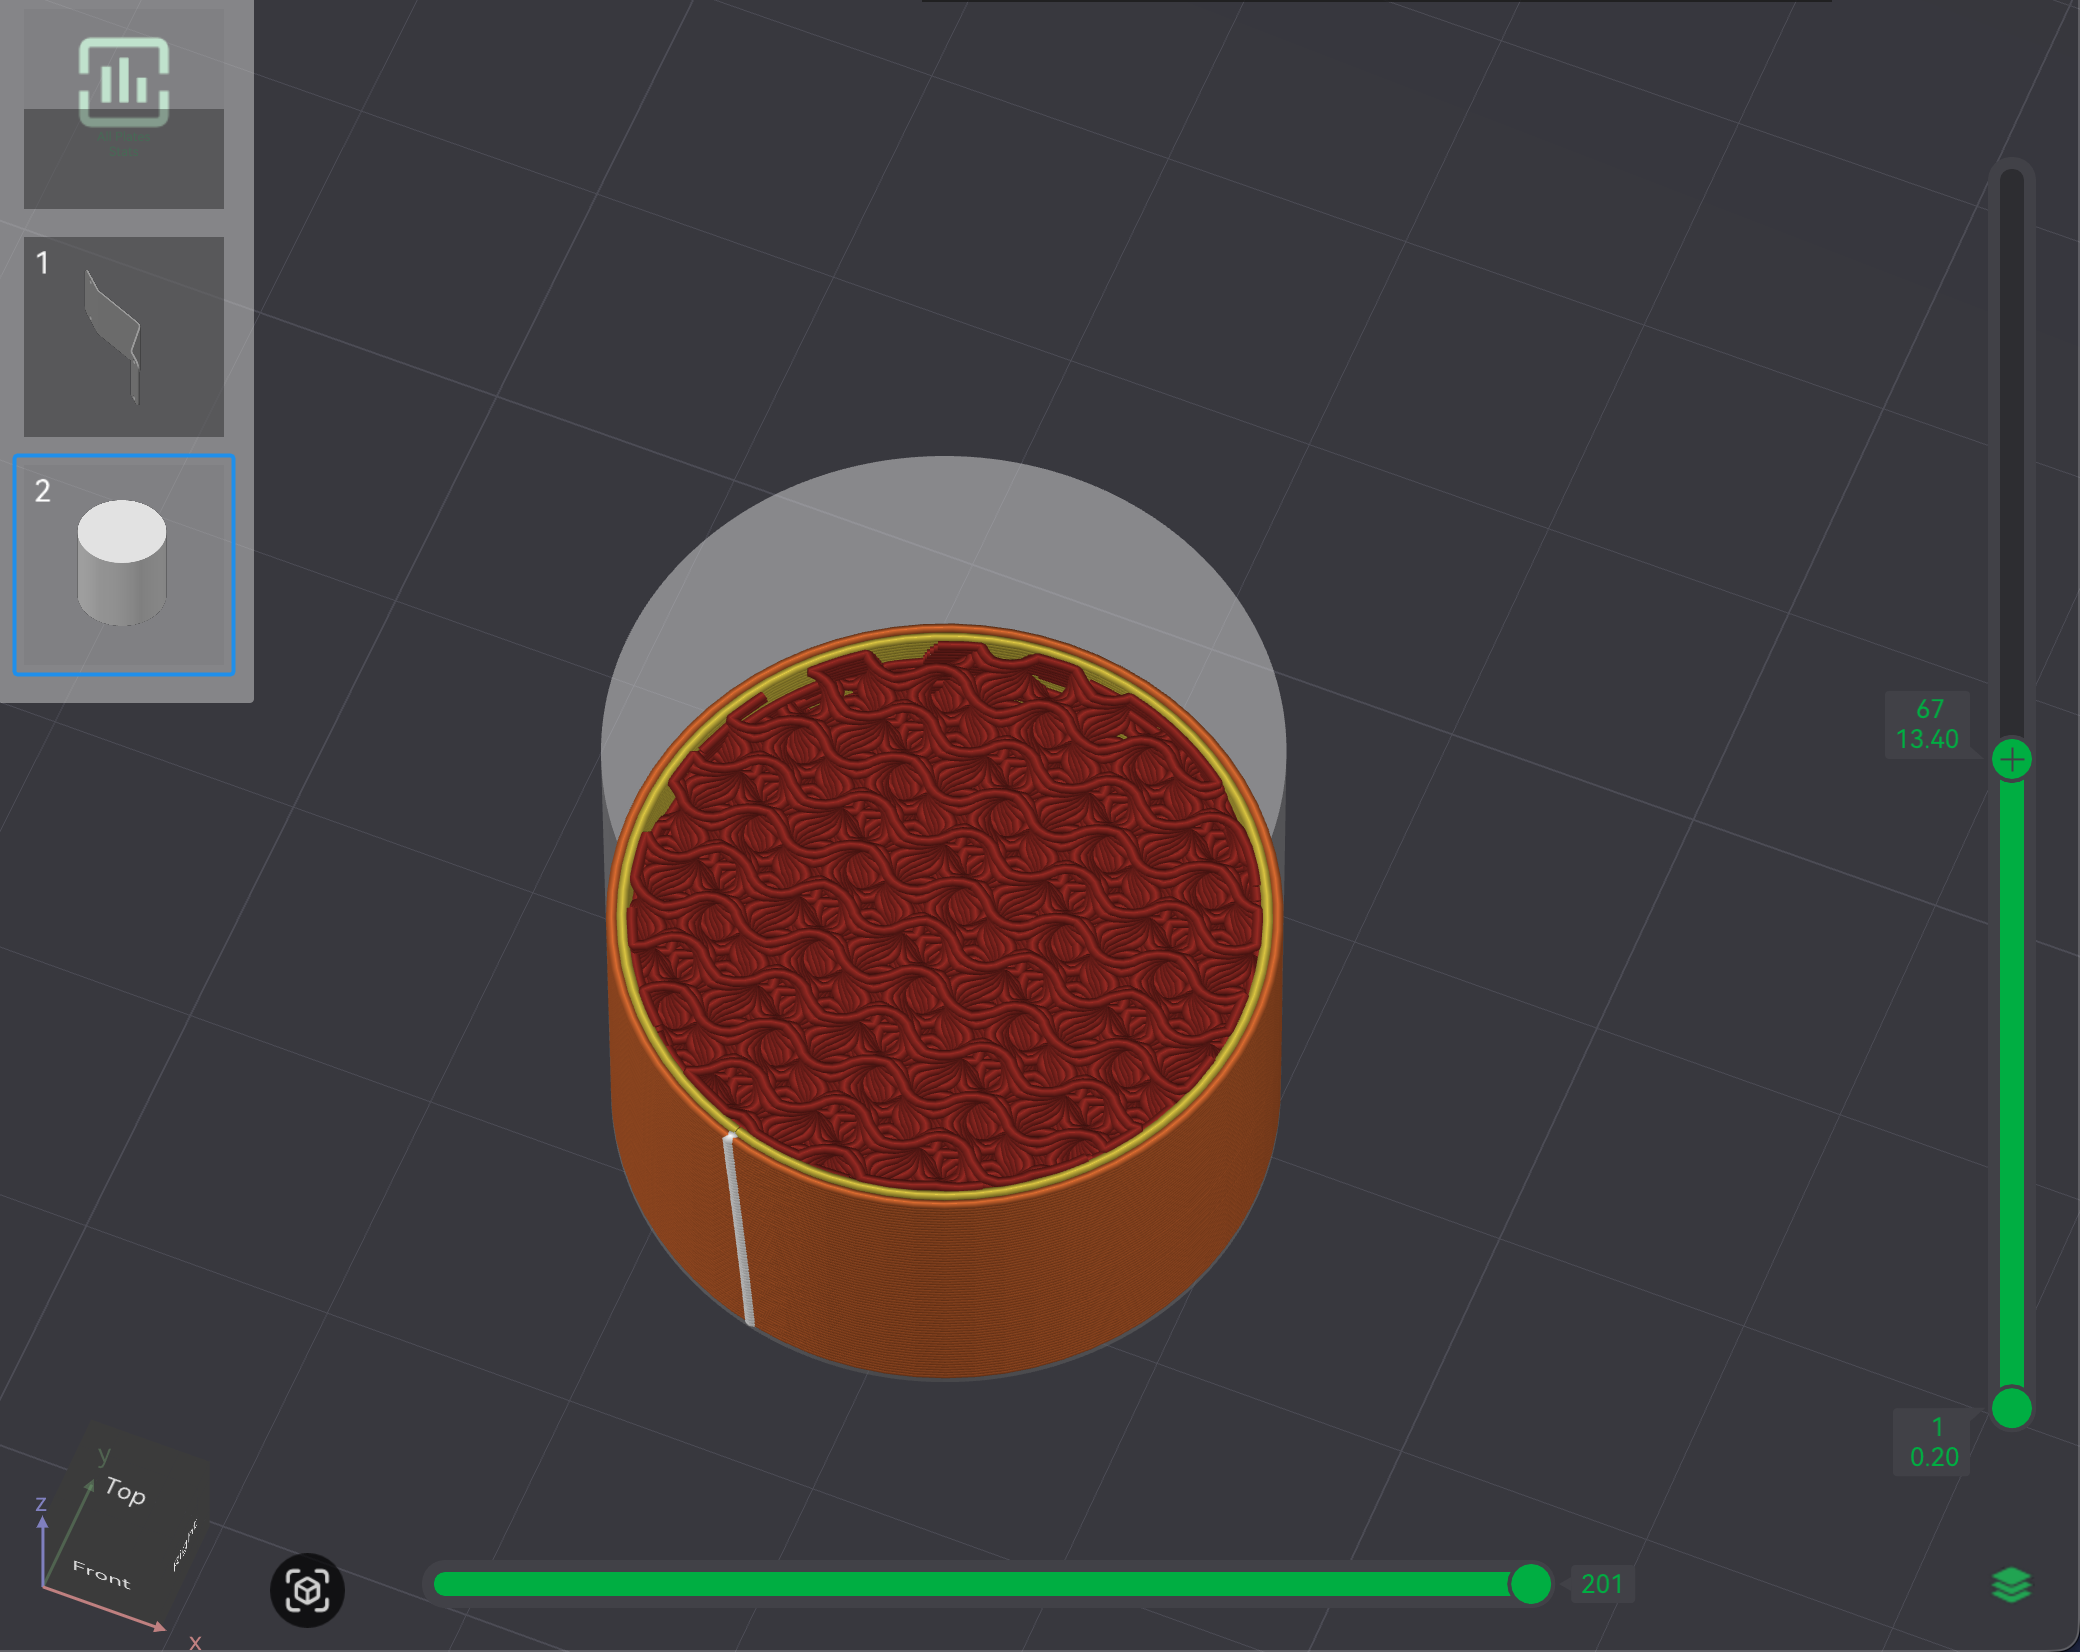
\includegraphics[width=0.49\textwidth]{gyroid}
    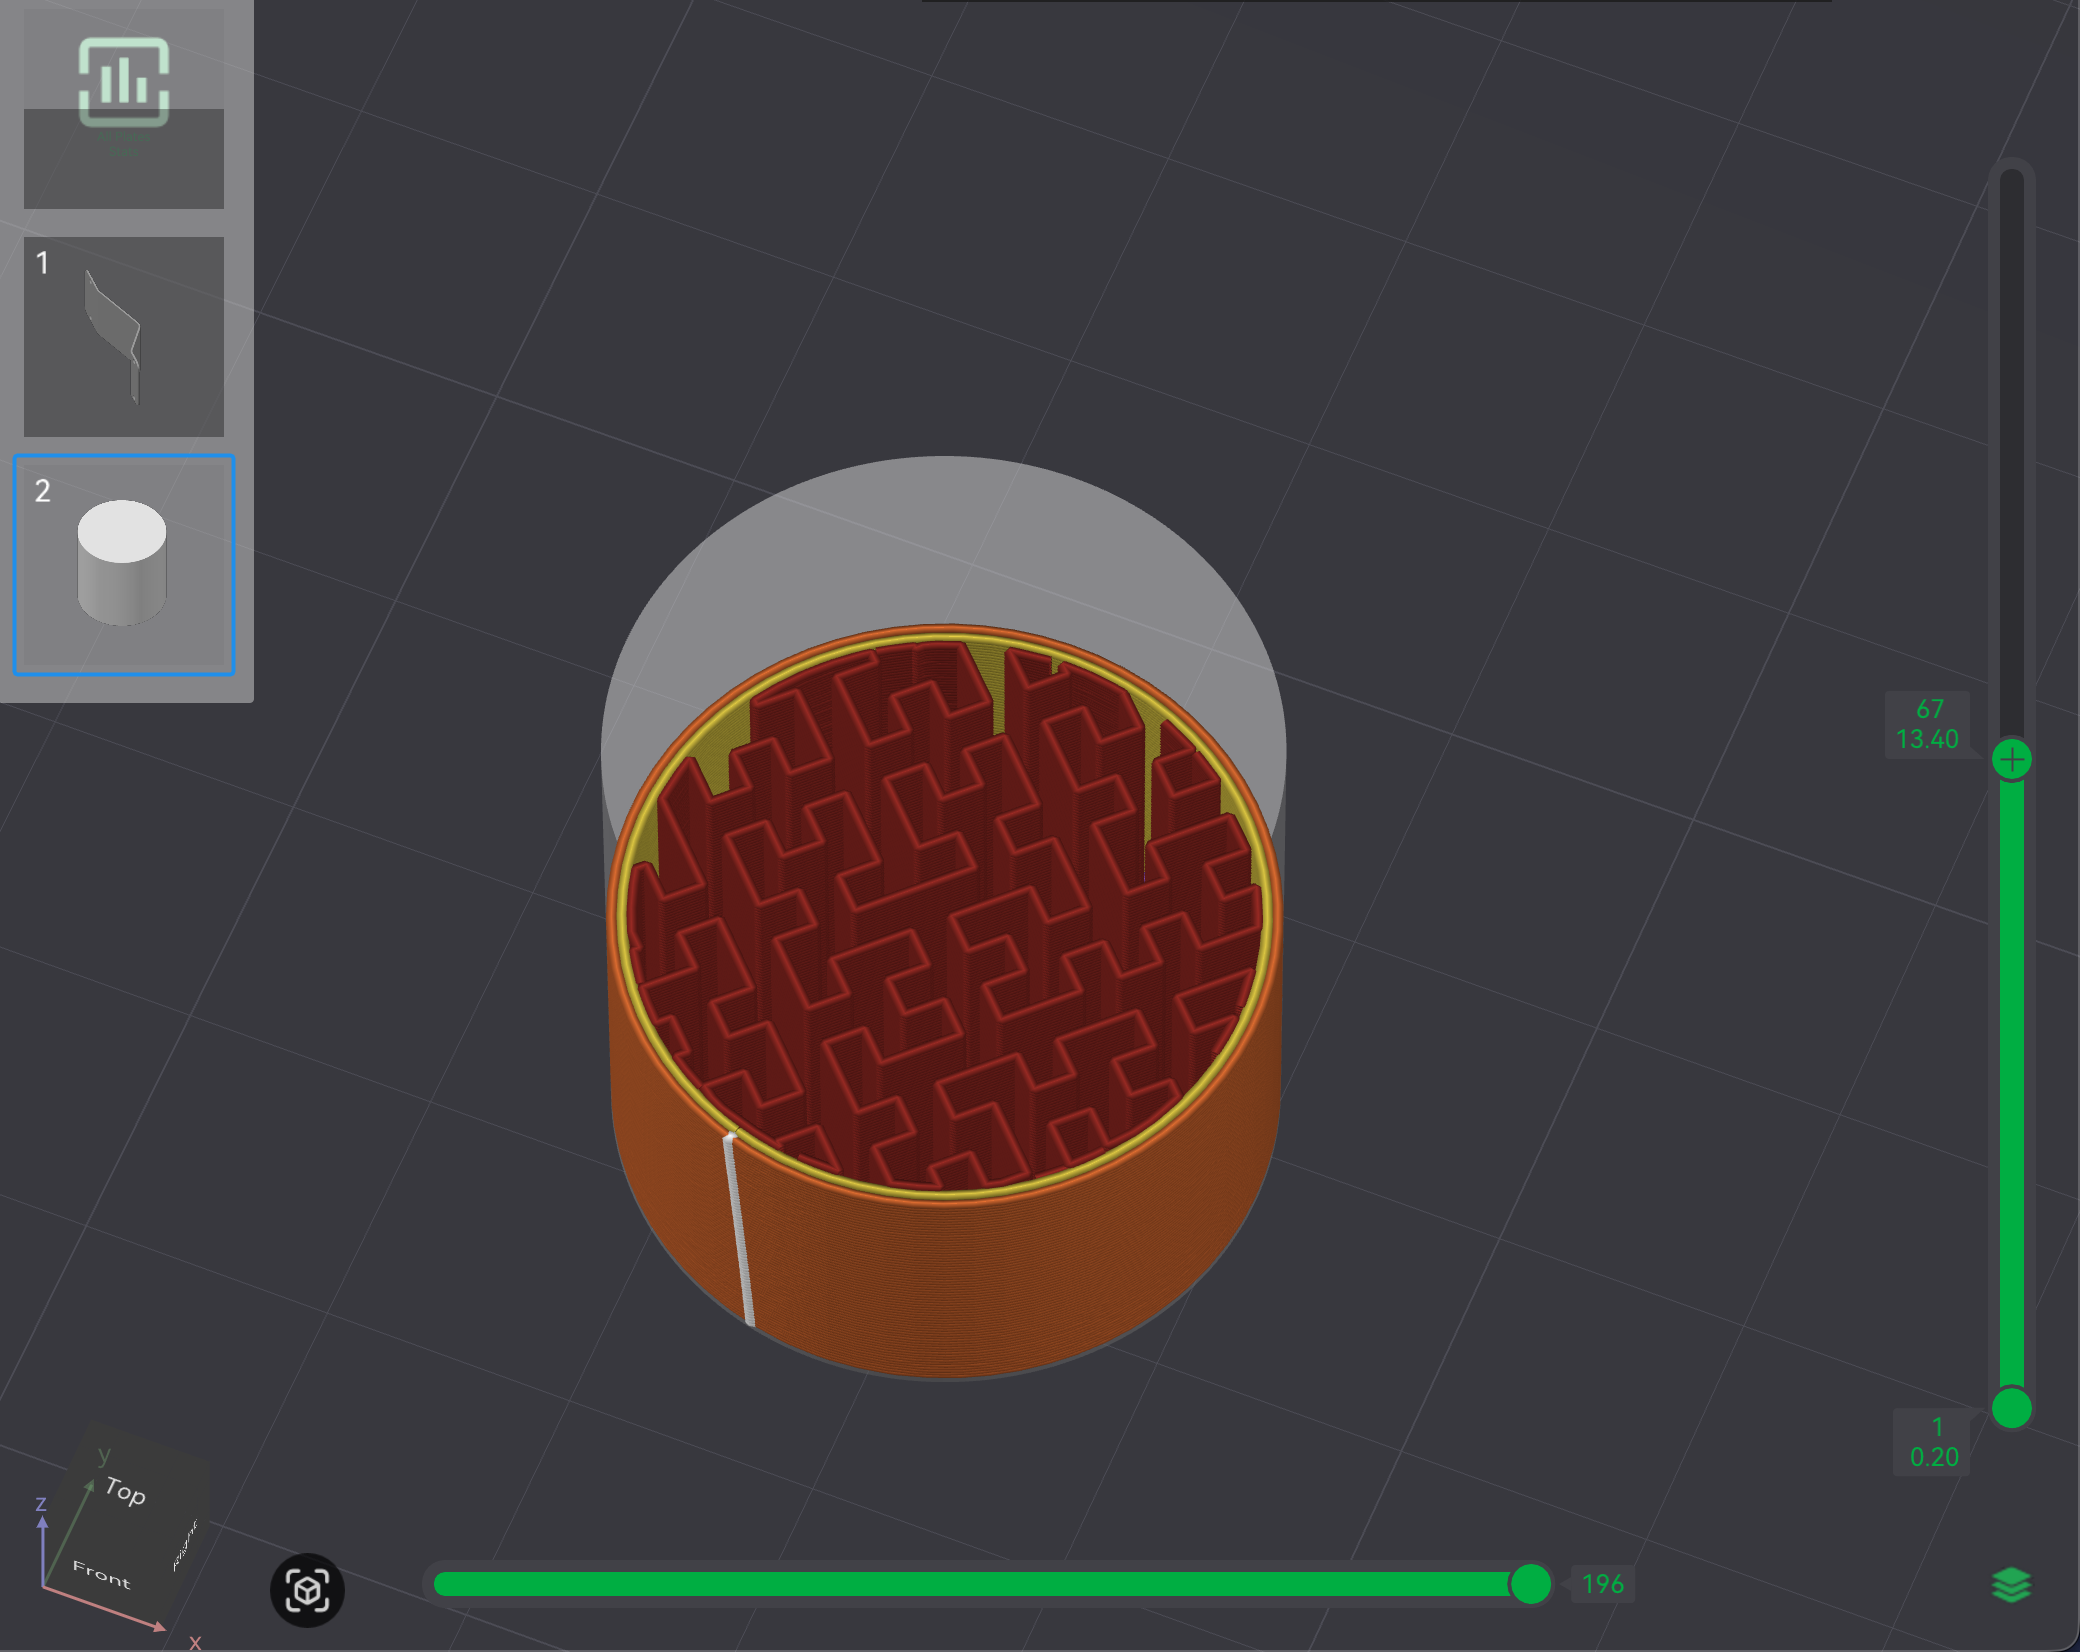
\includegraphics[width=0.49\textwidth]{hilbert_curve}
    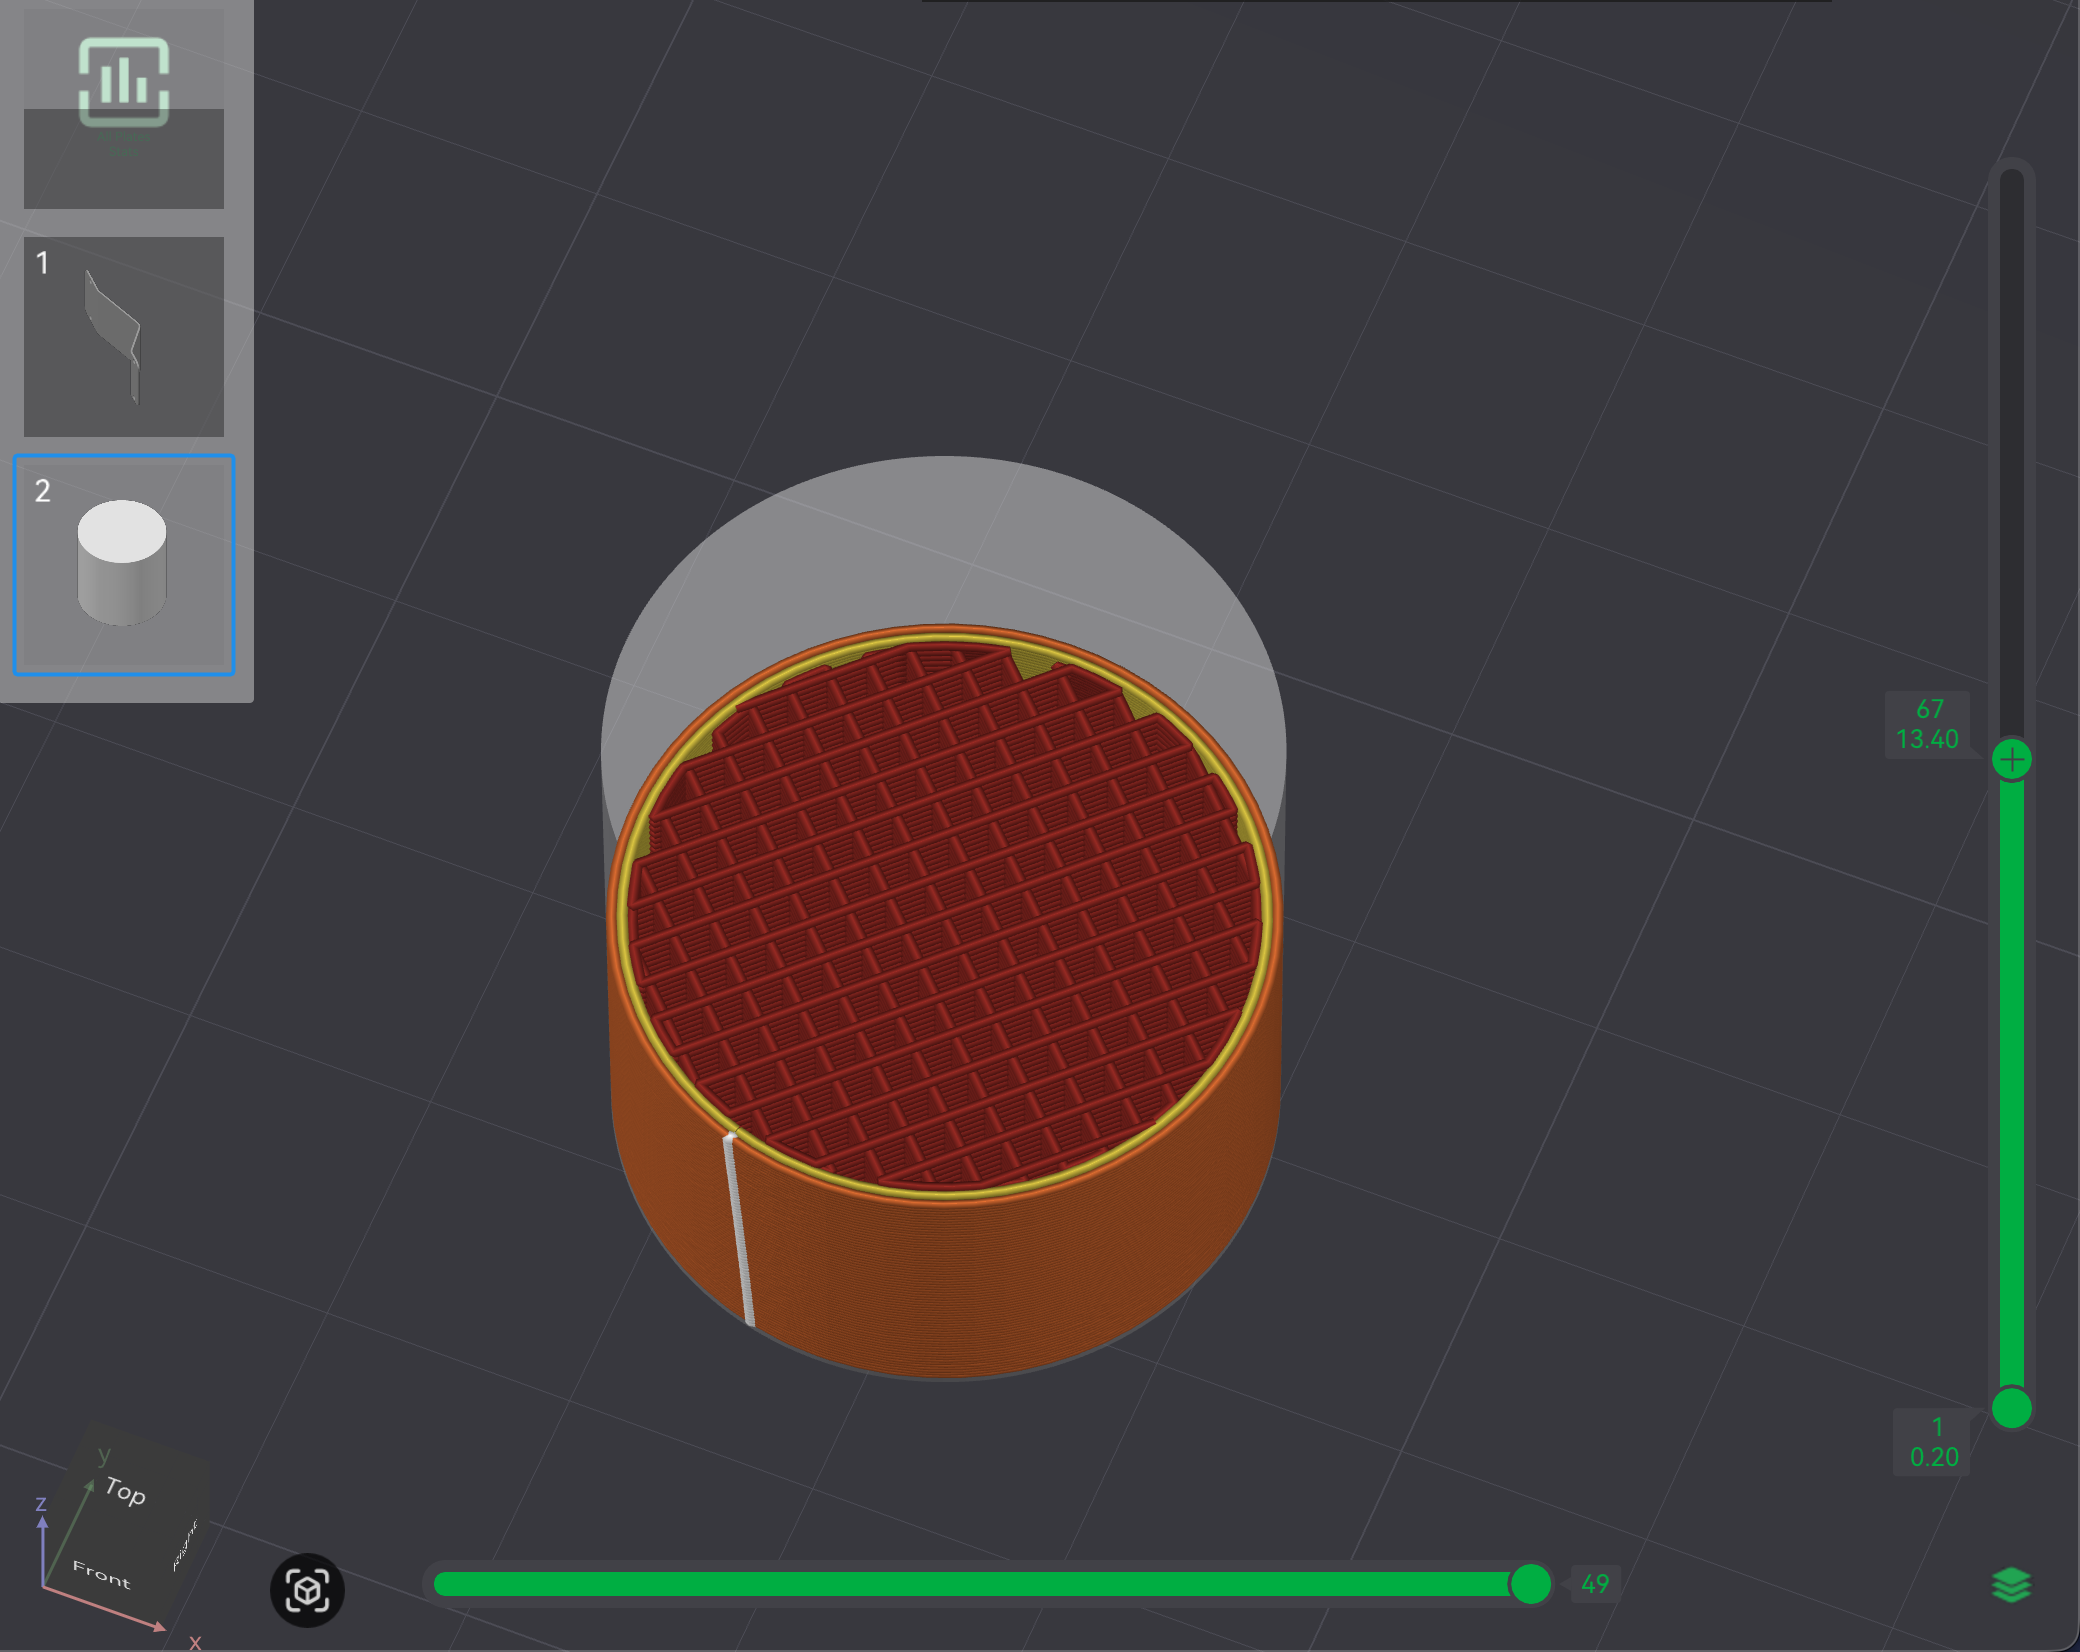
\includegraphics[width=0.49\textwidth]{rectilinear}
    \caption{Some infill patterns (25\%)}\label{fig:infill}
\end{figure}

\noindent
While these settings do make parts stronger, they can make them consume more materials and be heavier, as well as altering aesthetic properties on translucent and semi-translucent materials. My parts do not need to be strong, and so I only need 7\% infill and 2 wall loops, which will reduce both the time taken to print and the amount of material used.

\bigbreak\noindent
Some settings are there to make printing some objects possible or easier. Supports are a feature that are printed along with your model that are there for the molten plastic to rest on while it cools and hardens, which prevents sagging on overhangs. Once the printing is complete you can just break them off which sometimes leaves marks. Once enabled, the default settings for supports are usually fine and do not need to be configured.

\begin{figure}[ht]
    \centering
    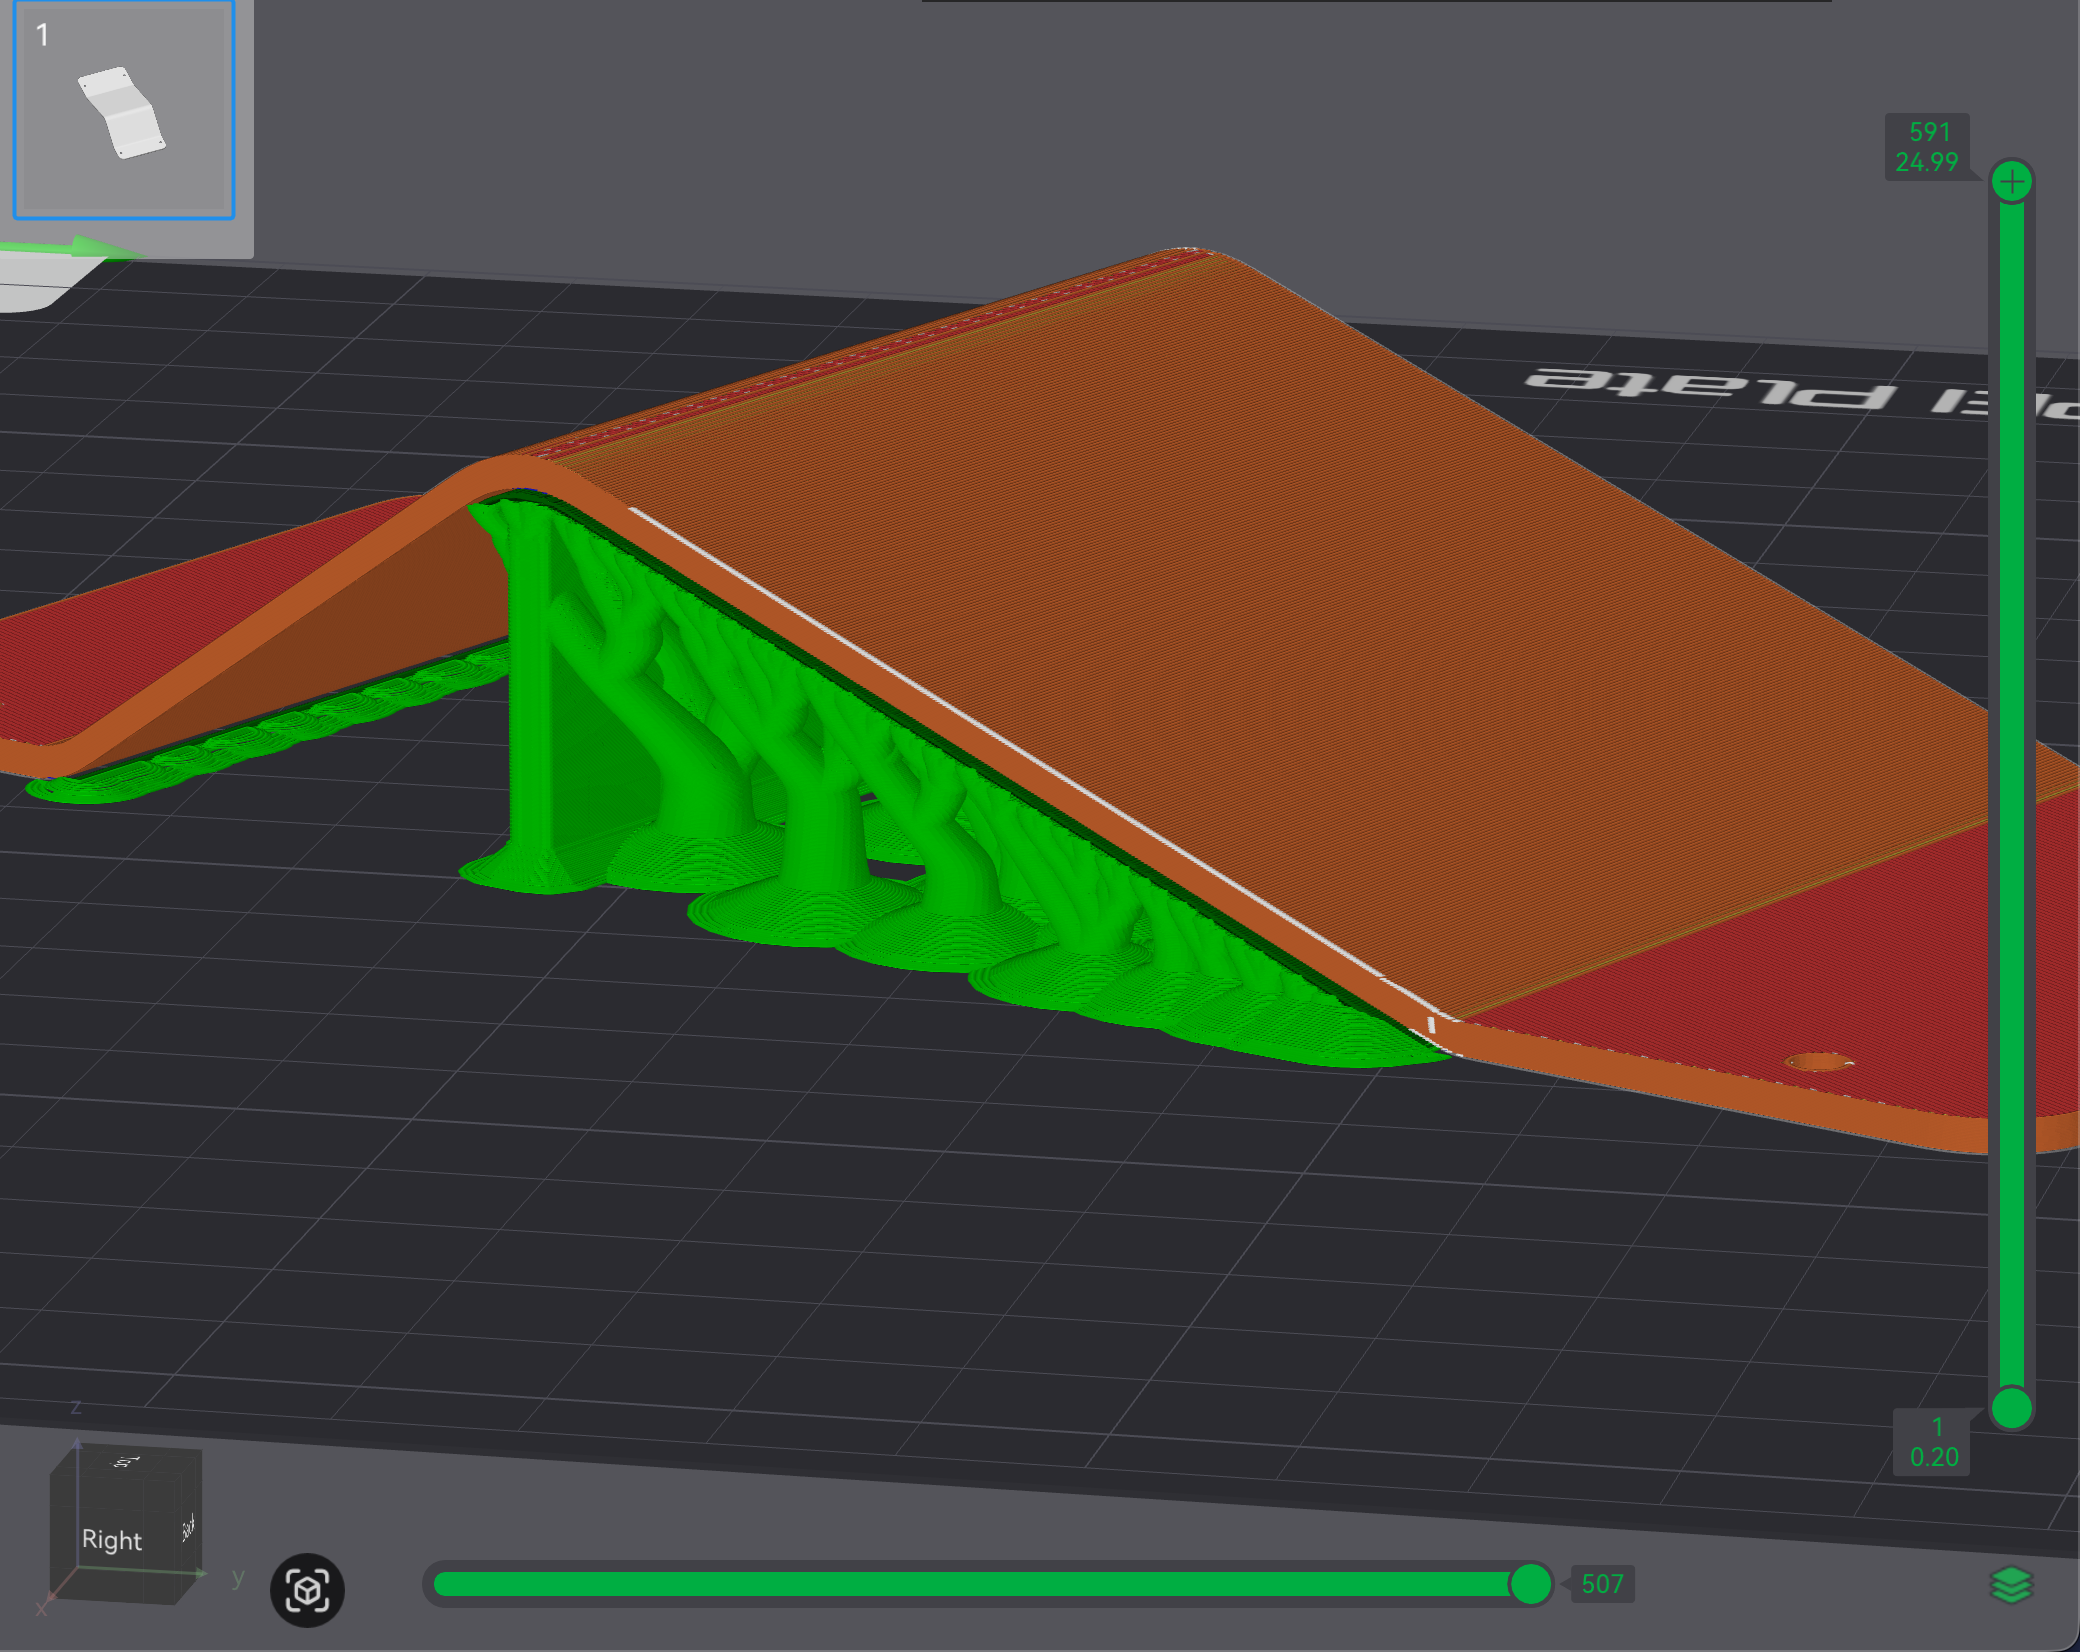
\includegraphics[width=0.49\textwidth]{supports}
    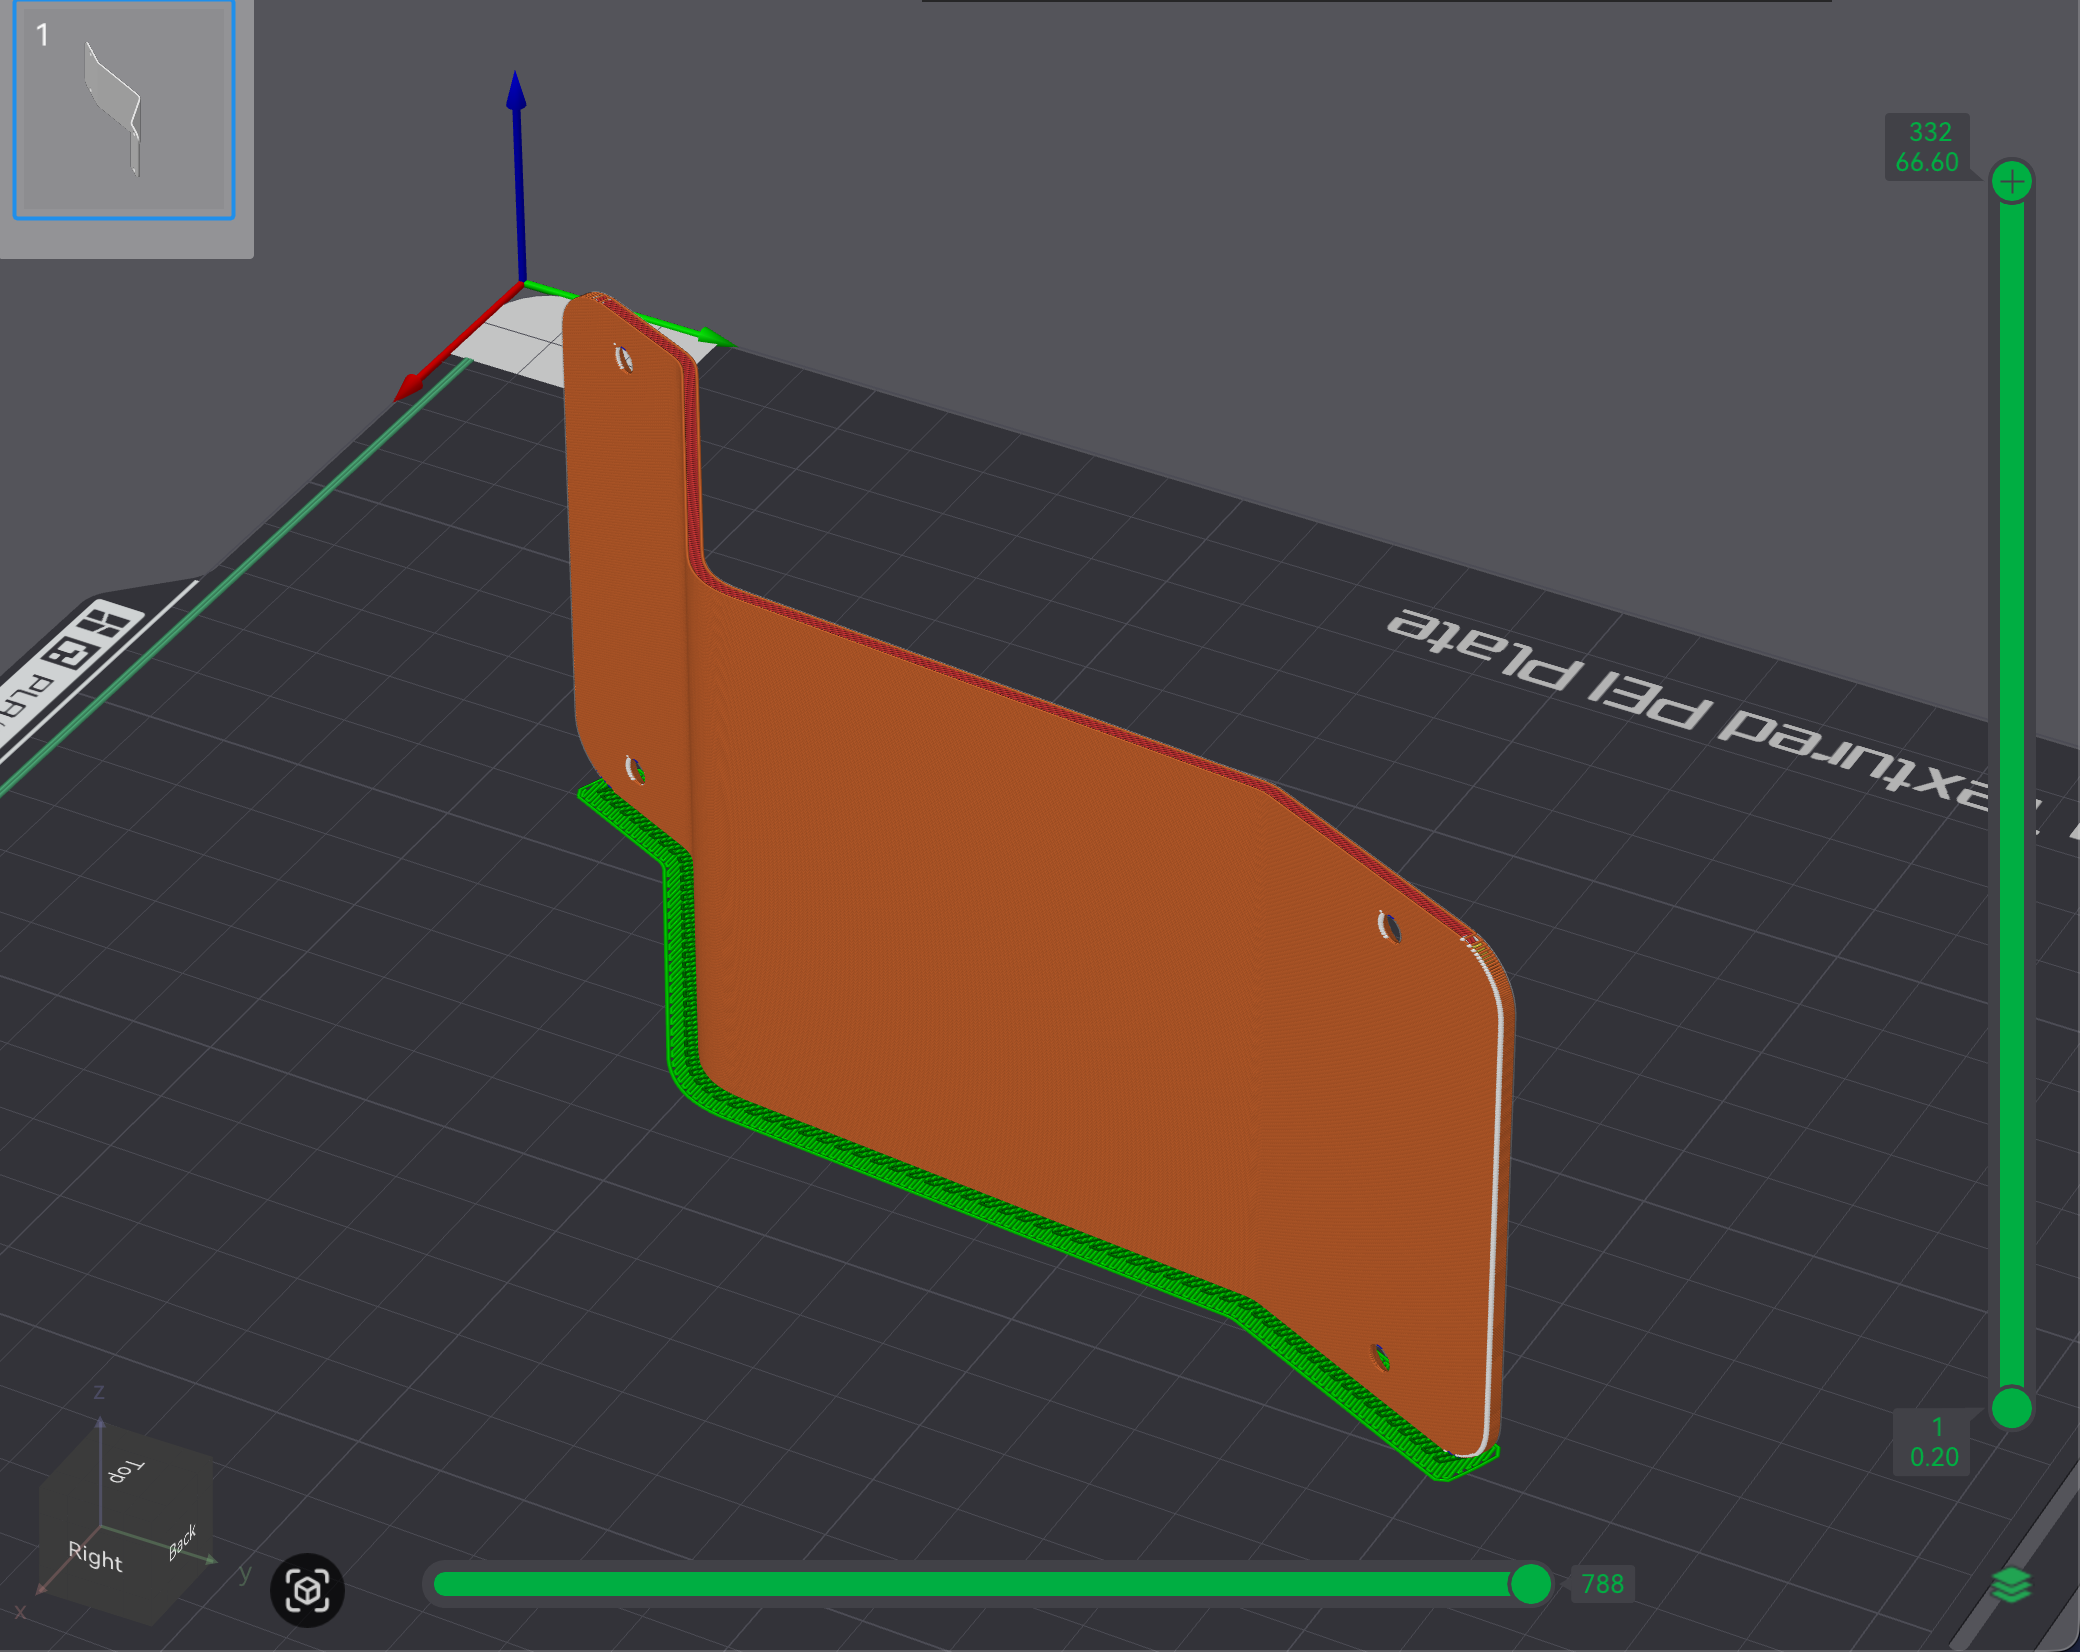
\includegraphics[width=0.49\textwidth]{raft}
    \caption{Tree, normal, $30^{\circ}$ threshold (left) \& 2 raft layers (right)}
\end{figure}

\bigbreak\noindent
Supports can dramatically increase the amount of material used and the print time which is why they should be avoided when possible.

On this model, since the orientation I am using has no overhangs, I do not need to enable supports. The other two models will require supports.

\bigbreak\noindent
However, a print will fail if it detaches from the print bed because the nozzle will be following the instructions it was given, printing onto where the model was. For models with a low contact area on the bed, rafts can be added. They have the same idea as supports, where they break off when the model has finished printing, but they instead just add a few loops of rings around the base of the model on the first few layers to increase the surface area. Rafts add very little print time and material to the print and usually do not leave a mark, which makes them fine to use when they are needed.

\bigbreak\noindent
A material needs to be chosen to print objects out of. You can either set what filament will be in the external spool, or, in my case, have filament automatically detected inside the Automatic Material System (AMS), and select it. Materials can have different physical or aesthetic properties such as temperature resistance, UV resistance, and colour.

\bigbreak\noindent
Bambu Studio also can automatically choose variables including print speed, flow rate, and fan speeds for a specific material which are very optimised for their printers which, in most cases, do not need changing. My print is does not contain any complex geometry that would require any special variables and so I decided that the default settings would be sufficient.

\bigbreak\noindent
Once sliced, Bambu Studio can automatically send the gcode wirelessly to the printer and begin a print, but first you need to make sure that the machine is ready.

\subsection{Machine preparation}

The machine needs filament loaded before a print starts to print with. I own an AMS, which makes this very easy. A roll can be placed on a slot and filament fed into the corresponding inlet. The machine will grab the filament and pull it some of the way through the system, to check for a Bambu NFC tag inside the spool for automatic detection and for weight estimation to tell you approximately how much of a roll is left.

The print bed also needs to be level so the toolhead will be able to print with an equal distance from the bed at any point, otherwise print failures from lost adhesion are more common. Luckily, Bambu Lab printers have an automatic bed leveling option that can be set while sending a print, that will add around 5 minutes to a print time, but ensure that the bed is fully level by probing it with the nozzle at different points and making adjustments if needed.

\bigbreak\noindent
Most 3D printers also support several different size nozzles, which can be swapped for different print results. A smaller nozzle will increase the amount of detail but will hugely increase the print time and decrease print strength, and also increase the chance of clogging. A larger nozzle does the opposite of these. I decided to use the nozzle that came with my printer, which is a 0.4mm nozzle, which is standard for regular prints and would be a much better use of my time, as opposed to my 0.2mm nozzle which is only for things that require high detail. 

\section{Production}

To begin a print, gcode is downloaded onto the printer and it begins execution.

\subsection{gcode Overview}

The printer will be sent the gcode file before printing starts, and it will be stored in an SD card. At print time, it will be read and interpreted into machine code and run on a microcontroller, which will send signals to motors and heating elements.

gcode commands consist of commands (M or G) and optional parameters (coordinates, temperatures, \ldots). Some examples of code would be:

\begin{minted}{gcode}
    M1 S50  ; sets some parameter on some machine function
    G1 X0 Y0 F0 ; move to 0, 0 with a feedrate of 0 mm/minute
\end{minted}

\noindent
Real gcode snippets generated for my Bambu P1S can be found below.

\subsection{Preproduction}

Before preproduction began, I made sure to keep my hands out of the chamber and away from any hot or moving pieces. I also opened my window and turned on a fan, which, along with the carbon air filter in the exhaust of the printer, would clean and provide airflow for the toxic air.

\bigbreak\noindent
First, all the components need to be heated up to the correct temperature. The gcode code to change the heatbed temperature is \mintinline{gcode}|M140 S[temperature]|, which is usually followed by an \mintinline{gcode}|M190 S[temperature]| to wait for the temperature to be reached. My printer does not have a chamber heater, since it was upgrade from a P1P, so the only other part that needs heating is the nozzle. There are two commands for changing the nozzle temperature, with \mintinline{gcode}|M109 S[temperature]| being synchronous, as opposed to \mintinline{gcode}|M104 S[temperature]|.

\bigbreak\noindent
This is the gcode to load filament from the AMS:

\bigbreak\noindent
\mintinline{gcode}|M620 S0A|: Begin AMS transaction

\noindent
\mintinline{gcode}|M109 S220|: Blocking set nozzle temp to $220^{\circ}$C

\noindent
\mintinline{gcode}|G1 X120 F12000|: Move toolhead to X120 with a feedrate of 12,000mm/minute

\noindent
\mintinline{gcode}|G1 X20 Y50 F12000|: Move toolhead to X20 Y50 with a feedrate of 12,000mm/minute

\noindent
\mintinline{gcode}|G1 Y-3|: Move toolhead to Y-3 (into filament cutter)

\noindent
\mintinline{gcode}|T0|: Tell AMS to swap roll

\noindent
\mintinline{gcode}|G1 X54 F12000|: Move toolhead to X54 with a feedrate of 12,000mm/minute

\noindent
\mintinline{gcode}|G1 Y265|: Move toolhead to Y265 (over purge chute)

\noindent
\mintinline{gcode}|M400|: Wait for AMS

\noindent
\mintinline{gcode}|M621 S0A|: End AMS transaction

\bigbreak\noindent
And one to ensure the nozzle is clean.

\begin{minted}{gcode}
M73 P15 R29
G1 X70 F9000
G1 X76 F15000
G1 X65 F15000
G1 X76 F15000
G1 X65 F15000
G1 X80 F6000
G1 X95 F15000
G1 X80 F15000
G1 X165 F15000
M400
M106 P1 S0
\end{minted}

\bigbreak\noindent
It moves the nozzle back and forth over the nozzle wiper rapidly to detach any sticking filament. It starts with an \mintinline{gcode}|M73 P[percentage] R[minutes]| to update the visual display for the user, followed by many \mintinline{gcode}|G1| commands to move the toolhead. It then waits for the queued commands to finish (\mintinline{gcode}|M400|) and turns the part fan off (\mintinline{gcode}|M106 P[fan] S[speed]|). Other preproduction steps are hidden behind proprietary macros in the gcode and are not viewable.

\subsection{Fabrication}

\begin{center}
    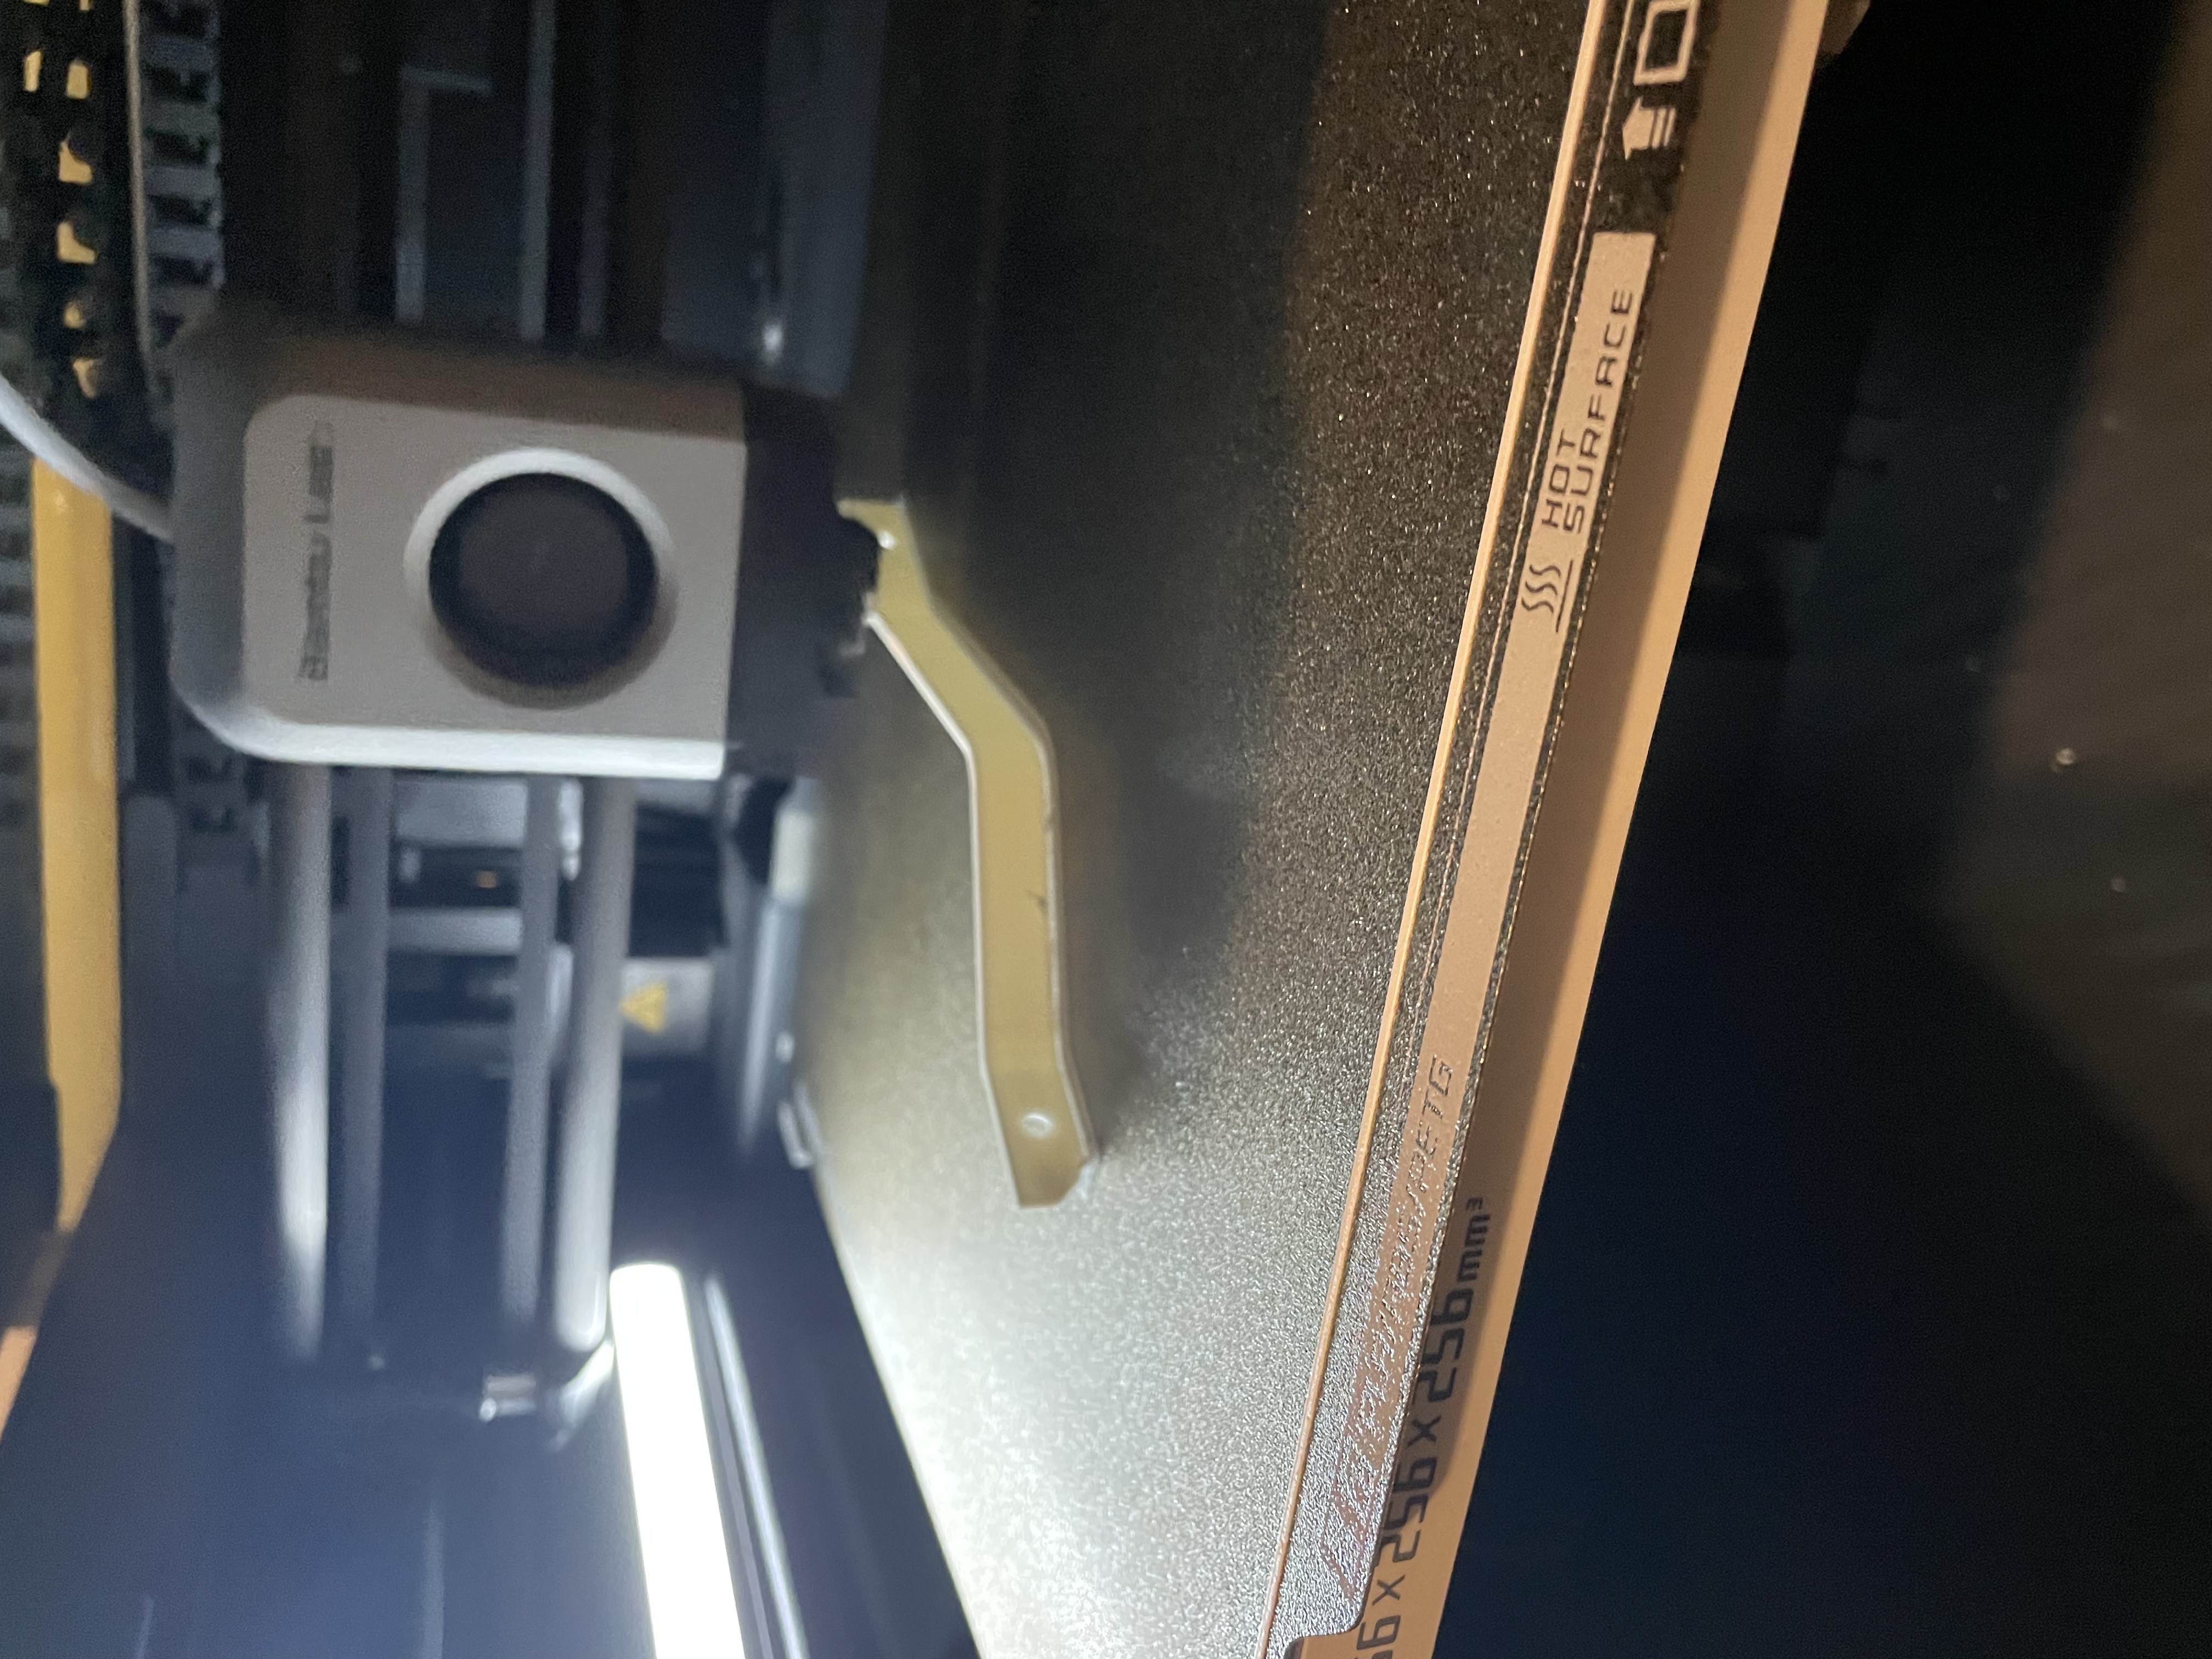
\includegraphics[width=0.6\textwidth, trim=0px 0px 750px 0px, clip, angle=-90]{mid_print}
\end{center}

\noindent
The gcode is much less interesting during the fabrication process, consisting nearly entirely of \mintinline{gcode}|G1| and \mintinline{gcode}|G3| commands to move the toolhead.

\bigbreak\noindent
When the print had completed, I opened the door and waited for temperatures to drop before putting my hands near the bed to retrieve the print. 

\section{Evaluation}

\begin{center}
    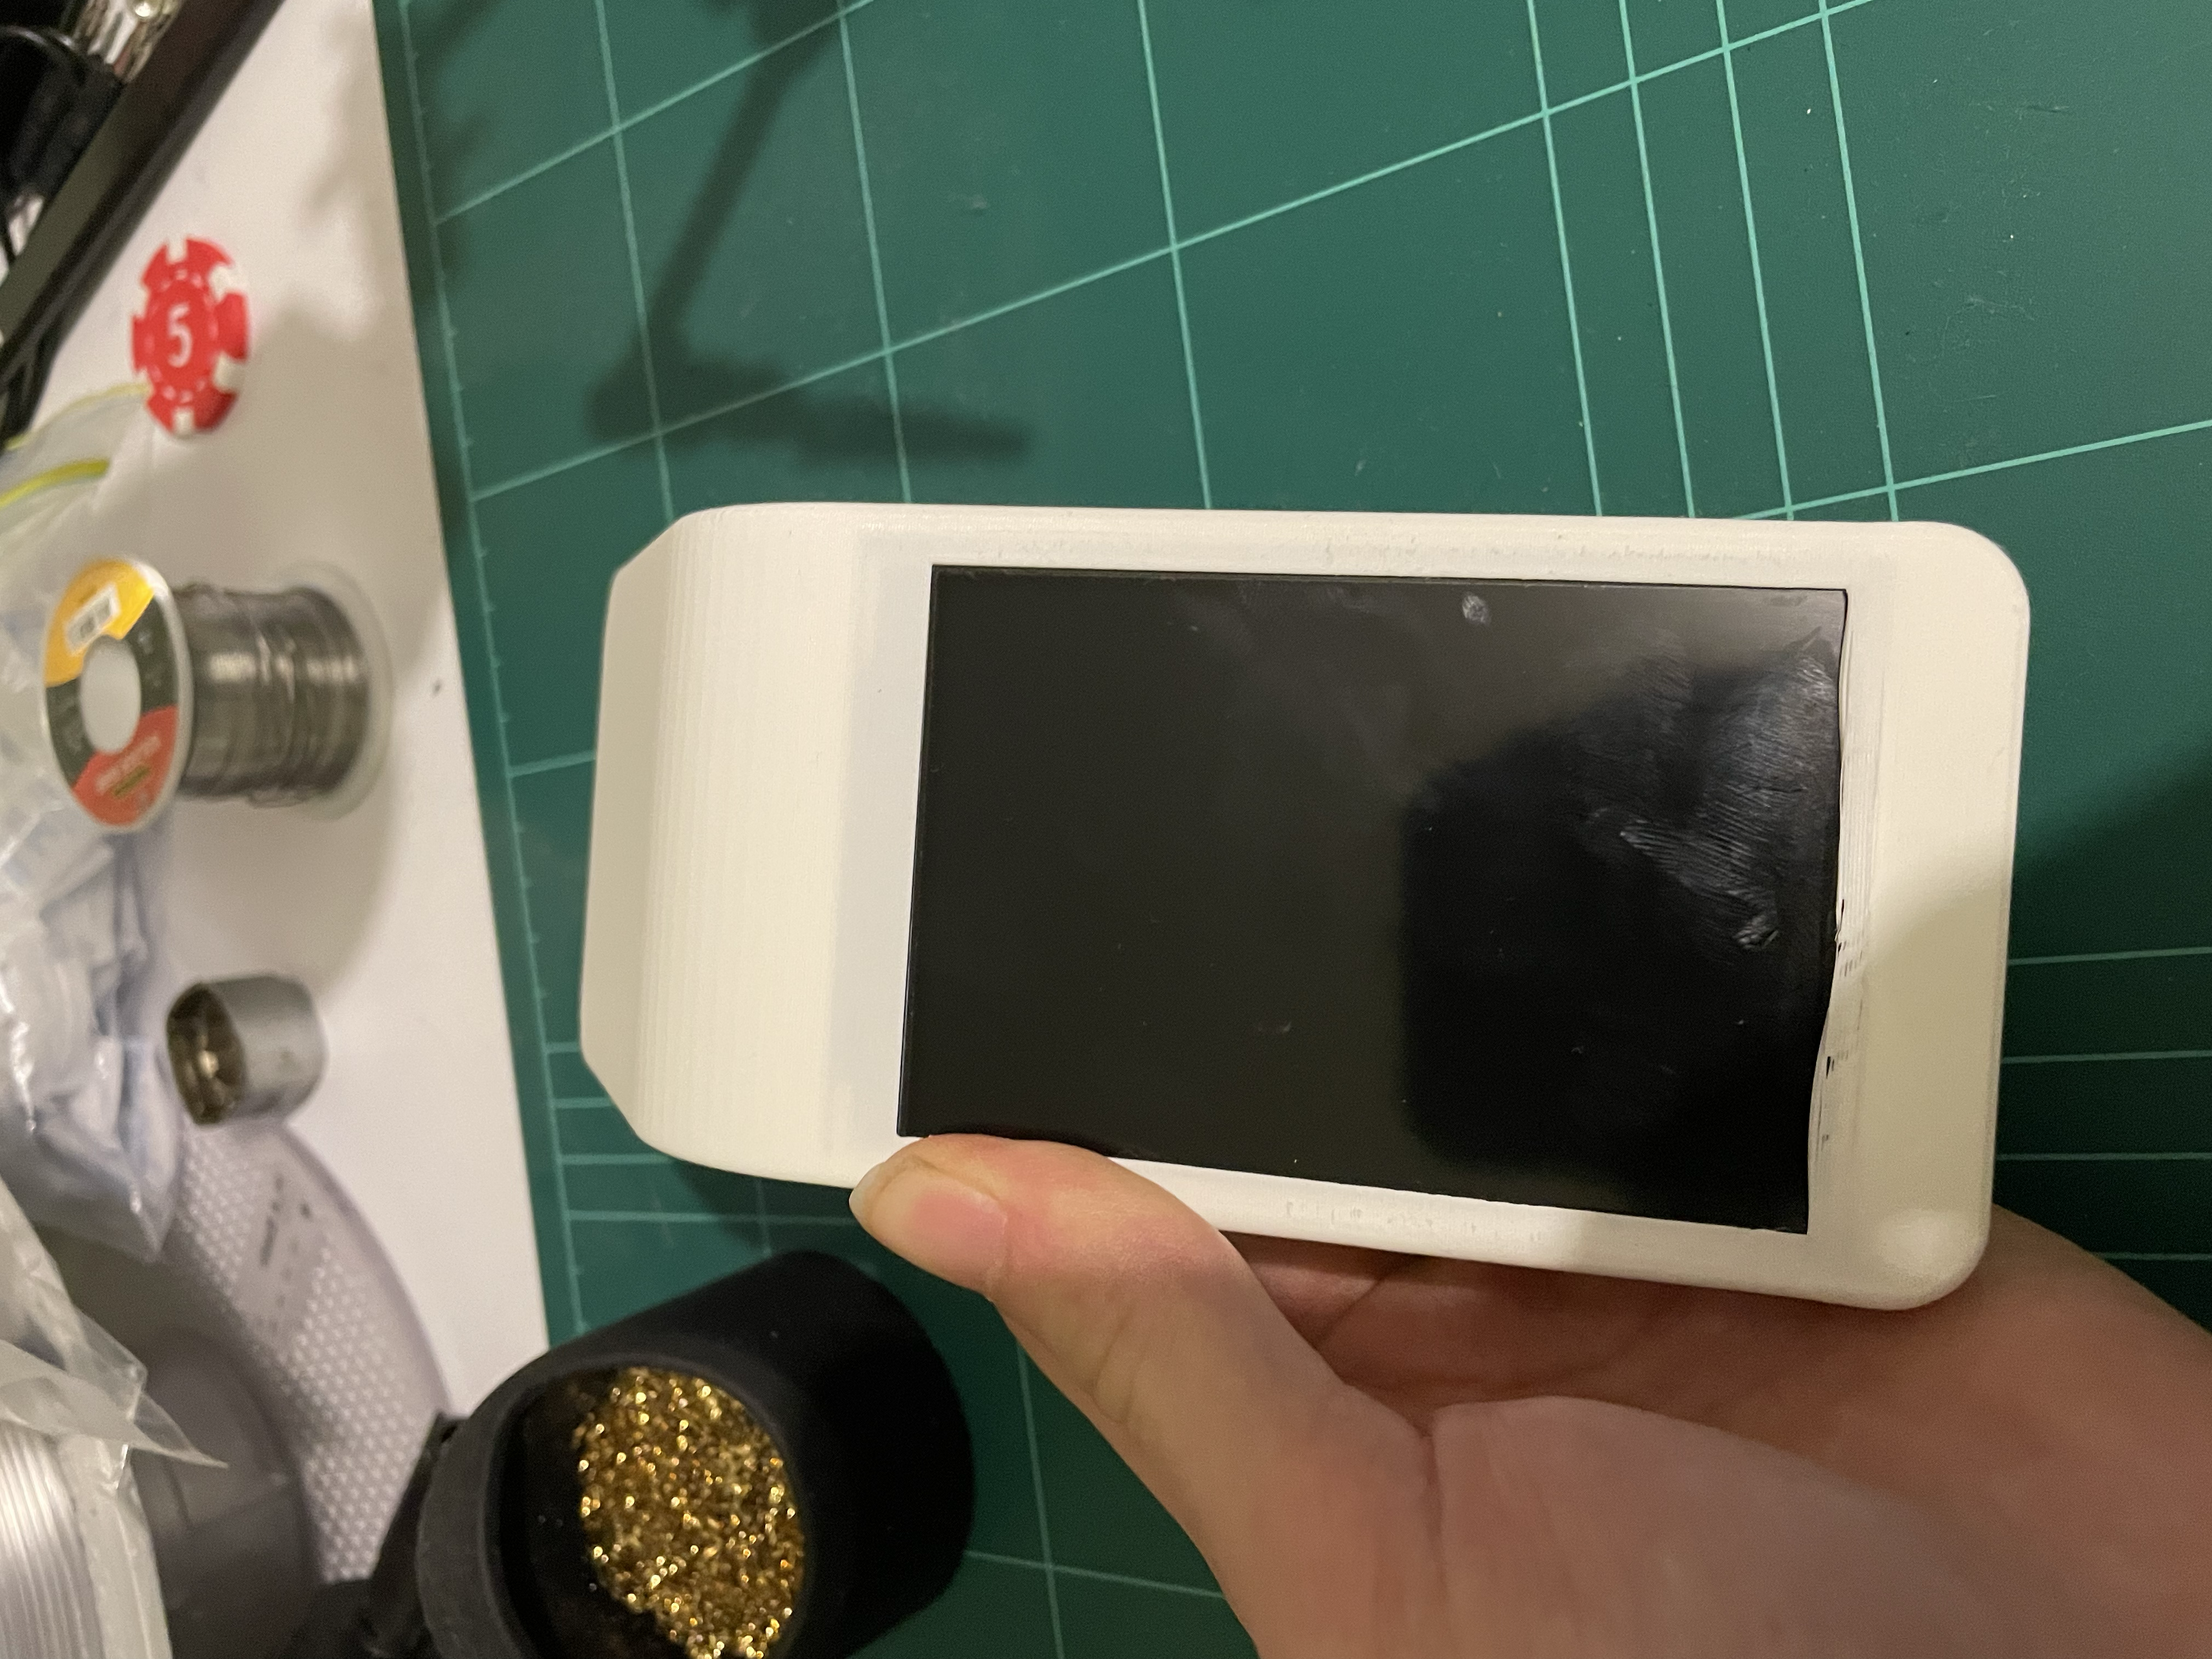
\includegraphics[width=0.6\textwidth, trim=500px 0px 0px 0px, clip, angle=-90]{final_product}
\end{center}

\noindent
To evaluate the success of the print, I made sure that the screw holes in each of the three pieces lined up and that the components fit inside of the shell. I also found that the tolerances I added for the screen resulted in a snug fit, which is perfect.

However, there was some sagging on the bottom of the screen (which was the underside during printing) which could be resolved by slowing down overhang print speed or by adding supports in that area.

\begin{center}
    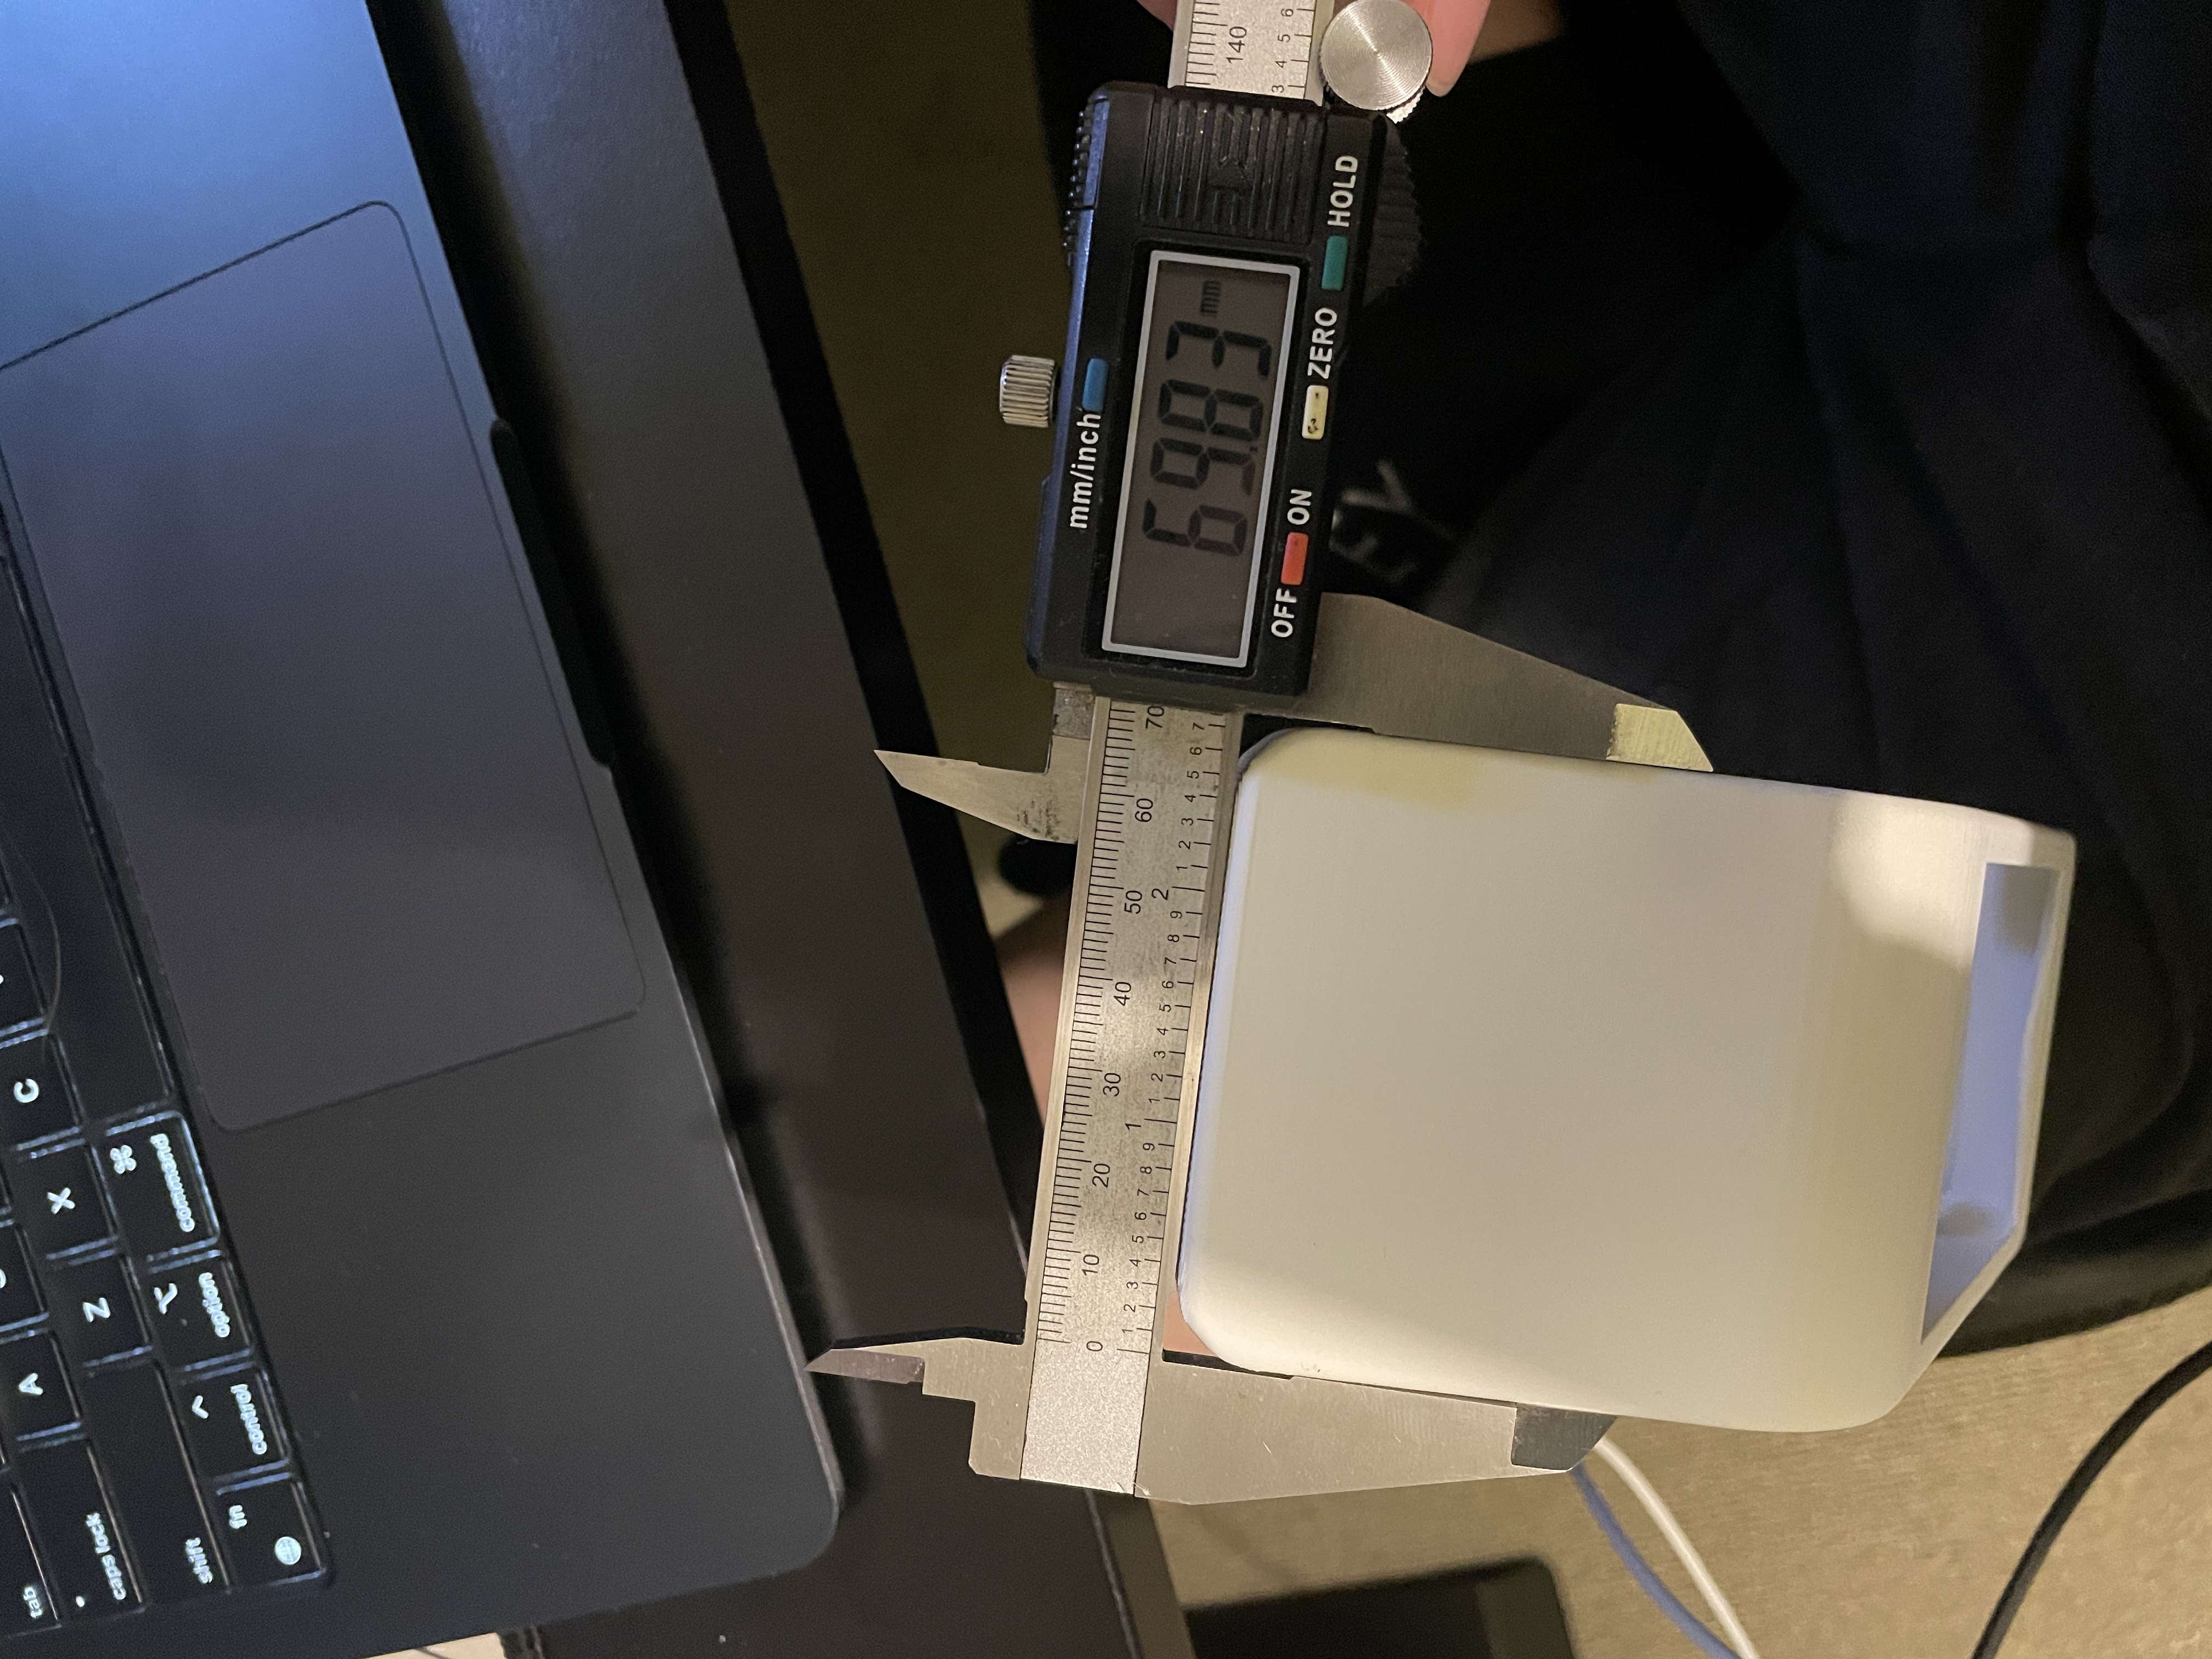
\includegraphics[height=0.49\textwidth,angle=-90]{measuring}
    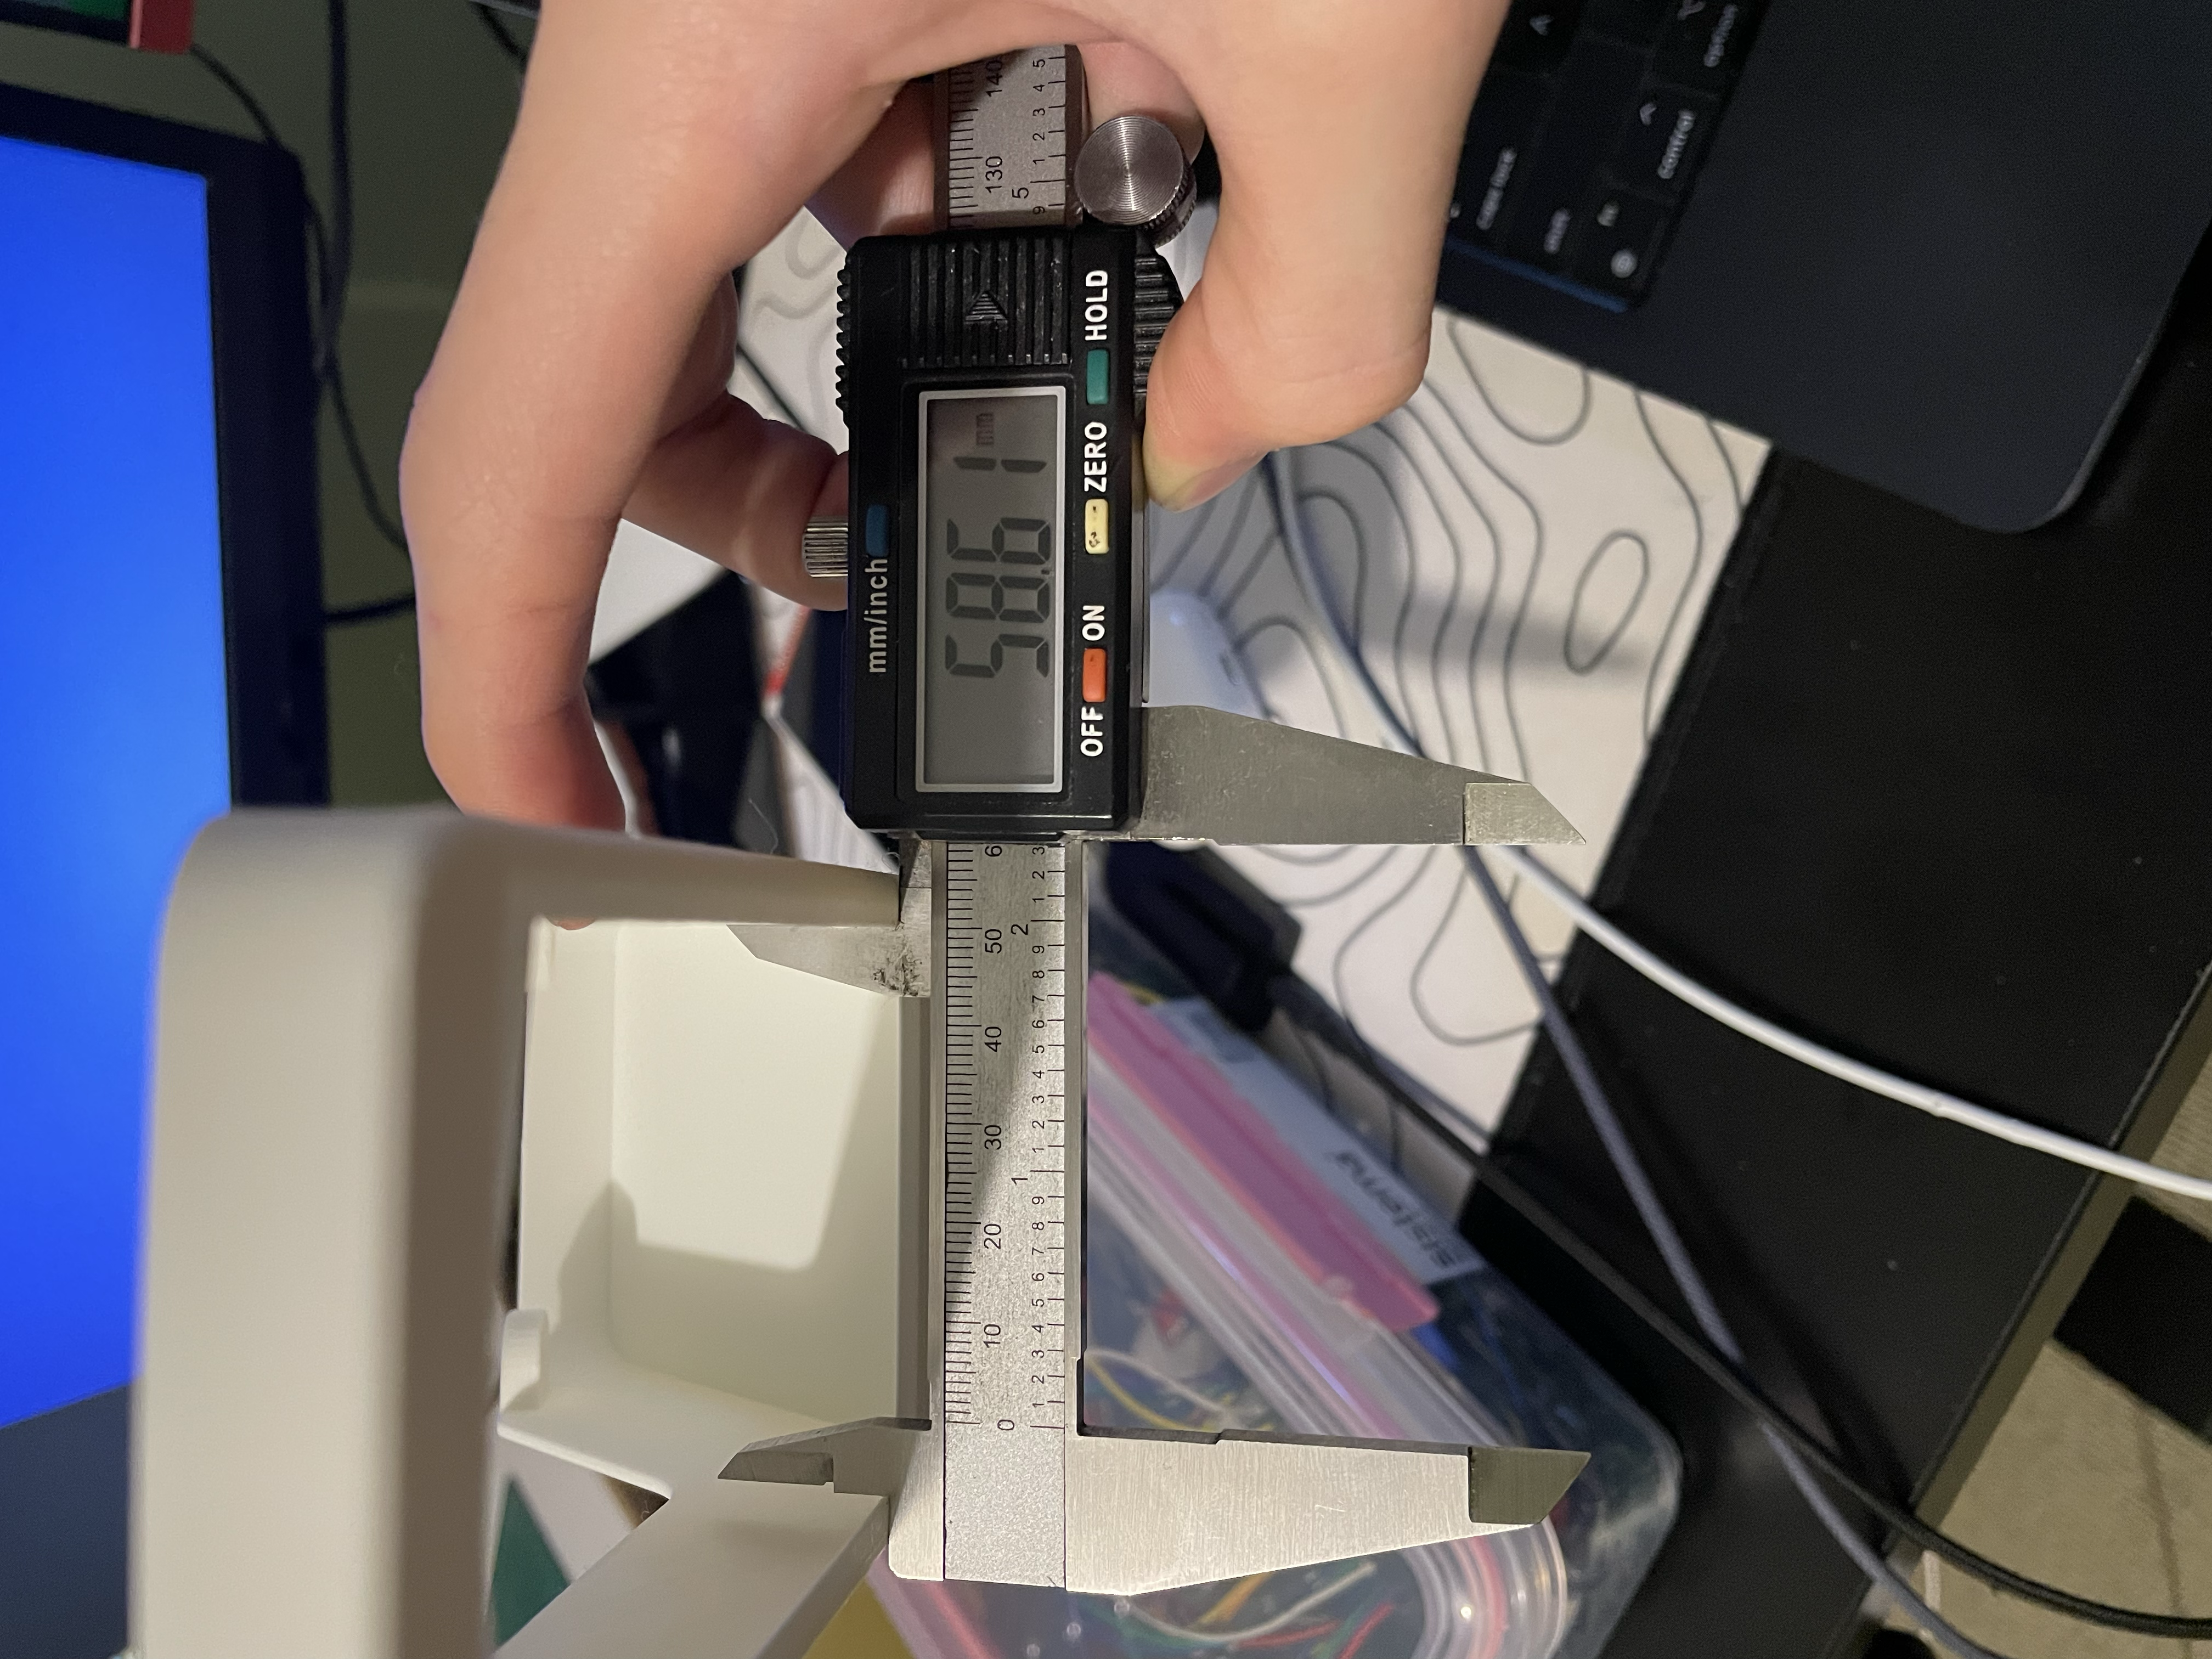
\includegraphics[height=0.49\textwidth,angle=-90]{measuring2}
\end{center}

Other measurements around the print were also measured using callipers and they were all within a 0.25mm of the computer measurements which showed that the printer was very accurate and my tolerances were around the right size.

\section{Recap}

\begin{list}{-}{}
    \item I designed a CAD model, keeping in mind the limitations of a 3D printer I identified (overhangs, shrinking, build volume, resolution), by adding tolerances and using shallow angles
    \item Prepared and calibrated (whether automatically or manually) the 3D printer for the print including bed leveling and filament loading
    \item Operated the machine with considerations for my safety, including staying clear of any hot or moving parts, and ensuring that the air would be safe to breathe by filtering the air and improving airflow in the room
    \item Evaluated my product against the specified requirements (screen fit, screw holes are aligned)
    \item Operated independently using my own equipment and showed accuracy by measuring using a precise instrument (callipers) on the initial design and evaluation, and copying measurements (including tolerances) into the appropriate areas.
    \item Economising time, materials, and effort by avoiding supports when possible, using AMS to automatically detect and load filament, and using a low infill percentage.
\end{list}

\end{document}